%! Suppress = MissingImport
%! Suppress = TooLargeSection
%! Suppress = SentenceEndWithCapital
%! Suppress = LineBreak
%! Suppress = MissingLabel
%! Suppress = Unicode

\documentclass[main.tex]{subfiles}

\begin{document}


    \section{Zasada indukcji matematycznej.}

    \begin{theorem}
        \textbf{Zasada indukcji matematycznej.} Niech T(n) - funkcja/forma zdaniowana zmiennej $n \in \mathbb{N}$. Jeżeli:
        \begin{enumerate}
            \item zachodzi $T(0)$
            \item $\forall n \in \mathbb{N} ~~ T(n) \Rightarrow  T(n+1)$
        \end{enumerate}
        to wtedy $T(n)$ jest prawdziwa dla każdego $n \in \mathbb{N}$.
    \end{theorem}

    \textbf{Schemat dowodu:}\\

    Niech $M = \{ n \in \mathbb{N}: ~ T(n) ~ zachodzi \}$, $M \subset \mathbb{N}$. Wtedy wg twierdzenia:
    \begin{enumerate}
        \item $\Rightarrow 0 \in M$
        \item $\Rightarrow n \in M \Rightarrow n+1 \in M$
    \end{enumerate}
    Zatem z \textbf{aksjomatu 5} wnioskujemy M = $\mathbb{N}$.

    \begin{theorem}
        \textbf{Aksjomat 5 liczb naturalnych (Peano)}. Niech będzie dany zbiór, którego elementami są liczby
        naturalne, o następujących właściwościach:
        \begin{enumerate}
            \item J jest elementem tego zbioru.
            \item Wraz z liczbą naturalną należącą do tego zbioru, należy do niego również jej następnik.
        \end{enumerate}
        Wtedy zbiór ten zawiera wszystkie liczby naturalne.
        $(Z \subset \mathbb{N}) \wedge (J \in Z) \wedge (\forall k \in \mathbb{N} k* \in Z) \Rightarrow Z = \mathbb{N}$.
    \end{theorem}

    \newpage

    \section{Porządki częściowe i liniowe. Elementy największe, najmniejsze, maksymalne i minimalne.}

    \begin{definition}
        \textbf{Częściowy porządek}. Niech X zbiór, $R \subset X \times X$ relacja. Wtedy R nazywamy \textbf{relacją częściowego porządku} w X
        $\Leftrightarrow$
        \begin{enumerate}
            \item R \textbf{zwrotna} ($\forall x \in X ~ xRx$),
            \item R \textbf{przechodnia} ($\forall x,y,z \in X ~ xRy \wedge yRz \Rightarrow xRz$),
            \item R \textbf{antysymetryczna} ($\forall x,y \in X ~ xRy \wedge yRx \Rightarrow x = y$).
        \end{enumerate}
        Piszemy: $\leqslant, \preceq, \prec gdy \neq$. \underline{Przykład:} $(\mathbb{R}, \leq)$, gdzie $x \preceq y \Leftrightarrow x \leq y ~ \forall x,y \in \mathbb{R}$.

        Wtedy $(\mathbb{R}, \preceq)$ jest cześciowym porządkiem.\\

        Jeżeli $(X, \mathbb{R})$ jest częściowym porządkiem, to elementy $x, y \in X$ nazywamy  \textbf{porównywalnymi}
        $\Leftrightarrow ~ xRy  \vee yRx$.\\

        \textbf{Diagram Hassego} - graf skierowany przedstawiający częściowy porządek w zbiorze, w odpowiedni sposób
        przedstawiony graficznie.
    \end{definition}

    \begin{definition}
        \textbf{Liniowy porządek}. Niech X zbiór, $R \subset X \times X$ relacja. Wtedy R nazywamy \textbf{relacją liniowego porządku} w X
        $\Leftrightarrow$
        \begin{enumerate}
            \item R \textbf{zwrotna} ($\forall x \in X ~ xRx$),
            \item R \textbf{przechodnia} ($\forall x,y,z \in X ~ xRy \wedge yRz \Rightarrow xRz$),
            \item R \textbf{antysymetryczna} ($\forall x,y \in X ~ xRy \wedge yRx \Rightarrow x = y$),
            \item R \textbf{spójna} ($\forall x,y \in X ~ xRy \vee yRx \vee x = y$).
        \end{enumerate}
    \end{definition}

    \begin{definition}
        Niech $\preceq$ jest relacją częściowego porządku wówczas element $m$ jest to:
        \begin{enumerate}
            \item \textbf{Element maksymalny}, jeśli $~~ \forall a \in A ~~ m \preceq a ~ \Rightarrow  ~ a = m$,
            \item \textbf{Element minimalny}, jeśli $~~ \forall a \in A ~~ a \preceq m ~ \Rightarrow  ~ a = m$,
            \item \textbf{Element największy}, jeśli $~~ \forall a \in A ~~ a \preceq m$,
            \item \textbf{Element najmniejszy}, jeśli $~~ \forall a \in A ~~ m \preceq a$.
        \end{enumerate}
    \end{definition}

    \newpage

    \section{Relacja równoważności i zbiór ilorazowy.}

    \begin{definition}
        Relację $R \subset X \times X$ nazywamy \textbf{relacją równoważości} $\Leftrightarrow$ relacja R jest:
        \begin{enumerate}
            \item \textbf{zwrotna} ($\forall x \in X ~ xRx $),
            \item \textbf{symetryczna} ($\forall x,y \in X ~ xRy \Rightarrow yRx$),
            \item \textbf{przechodnia} ($\forall x,y,z \in X ~ xRy \wedge yRz \Rightarrow xRz$).
        \end{enumerate}
    \end{definition}

    \begin{definition}
        Niech $R \subset X \times X$ będzie relacją równoważności, $X \neq \varnothing$, $x \in X$. \textbf{Klasą abstrakcji}
        elementu x (wzgledem relacji R) nazywamy:

        $[x]_{R} = \{y \in X: xRy\}$

        Element x nazywamy reprezentantem klasy abstrakcji $[x]_{R}$.
    \end{definition}

    \begin{definition}
        \textbf{Zbiorem ilorazowym} zbioru X przez relację R nazywamy zbiór wszystkich klas abstrakcji.

        $X/R = \{[y]_{R}: x \in X\} ~~ \subset X$
    \end{definition}

    \newpage

    \section{Metody dowodzenia twierdzeń: wprost, nie wprost, przez kontrapozycję.}

    Dla prawdziwości zdania:
    \begin{align*}
        p \Rightarrow q
    \end{align*}

    \begin{definition}
        \textbf{Dowód wprost}. Metoda dowodu wprost polega na założeniu, że p jest prawdą i pokazaniu, że wówczas q
        jest prawdą.
    \end{definition}

    \begin{definition}
        \textbf{Dowód nie wprost}. Metoda dowodu nie wprost opiera się na następującej tautologii rachunku
        zdań, zwanej prawem kontrapozycji:
        \begin{align*}
            (p \Rightarrow q) \Leftrightarrow (\neg q \Rightarrow \neg p).
        \end{align*}
        Zatem stosując tę metodę zakładamy, że q jest zdaniem fałszywym i pokazujemy, że p jest również
        zdaniem fałszywym.
    \end{definition}

    \begin{definition}
        \textbf{Dowód przez zaprzeczenie} Metoda dowodu przez zaprzeczenie opiera się na następującej tautologii rachunku
        zdań:
        \begin{align*}
            (p \Rightarrow q) ~ \Leftrightarrow ~ (\neg p \vee q) ~ \Leftrightarrow ~ \neg(p \wedge \neg q)
        \end{align*}
        Stosując to podejście zakładamy, że p jest prawdą a q fałszem i pokazujemy, że prowadzi to do sprzeczności,
        to znaczy, pokazujemy że $(p \wedge \neg q)$ jest fałszem.
    \end{definition}

    \newpage

    \section{Metody numeryczne rozwiązywania równań nieliniowych: bisekcji, siecznych, Newtona.}

    \subsection{Metoda połowienia (bisekcji)}

    \textbf{Założenia:}
    \begin{itemize}
        \item $f$ jest funkcją ciągłą w przedziale $[a,b]$,
        \item $f(a)f(b) < 0$.
    \end{itemize}
    Z własności Darboux funkcji ciągłych, funkcja f ma miejsce zerowe w przedziale $[a,b]$.

    \begin{definition}
        \textbf{Algorytm bisekcji} polega na obliczeniu $f(c_k)$, gdzie $c_k = \frac{a_k + b_k}{2}$ i zastąpieniu przez
        $c_k$ tej z liczb $a_k, b_k$ dla której funkcja $f$ ma taki sam znak.
        \begin{center}
            $(a_{k+1}, b_{k+1}) = (c_k, b_k)$ jeżeli $f(a_k)f(c_k) > 0$\\
            $(a_{k+1}, b_{k+1}) = (a_k, c_k)$ jeżeli $f(b_k)f(c_k) > 0$
        \end{center}
        Jeżeli $f(c_k) = 0$ to kończymy obliczenia.
    \end{definition}
    \begin{itemize}
        \item Metoda bisekcji jest \textbf{niezawodna}, ale \textbf{wolno zbieżna}.
        \item W każdym kroku szerokość przedziału jest dzielona przez dwa.
        \item Kryteria zakończednia obliczeń:
        \begin{itemize}
            \item osiągnięto dokładność $\delta: |e_n| < \delta$
            \item wartość funkcji jest bliska 0: $f(c_n) < \epsilon$
            \item wykonano M iteracji
        \end{itemize}
        \item Algorytm bisekcji w k-tej iteracji przybliża rozwiązanie $\alpha$ z \textbf{dokładnością:} $|x_k - \alpha| \leq \frac{|b - a|}{2^k}$.
    \end{itemize}


    \subsection{Metoda siecznych}

    \textbf{Założenia:}
    \begin{itemize}
        \item $f$ jest funkcją ciągłą w przedziale $[a,b]$,
        \item $f(a)f(b) < 0$.
    \end{itemize}

    \begin{align*}
        x_{k+1} = x_k - \frac{f(x_k)(x_k - x_{k-1})}{f(x_k) - f(x_{k-1})}
    \end{align*}
    gdzie $x_0 = a$, $x_1 = b$.

    \begin{itemize}
        \item W metodzie siecznych rezygnujemy z założenia, że funkcja na końcach przedziału ma różne znaki.
        \item Należy kontrolować zachowanie otrzymanego ciągu. \textbf{Może się zdarzyć, że metoda wyprodukuje ciąg rozbieżny!}
        \item korzyści płynące ze stosowania tej metody to zdecydowanie \textbf{szybsza zbieżność} ciągu iteracji, jeśli
        $x_n, x_{n+1}$ juz są dobrymi \textbf{przybliżeniami pierwiastka}.
    \end{itemize}

    \subsection{Metoda Newtona (stycznych)}

    \begin{align*}
        x_{n+1} = x_n - \frac{f(x_n)}{f'(x_n)}
    \end{align*}

    \textbf{Zmodyfikowana metoda Newtona:}
    \begin{align*}
        x_{n+1} = x_n - \frac{f'(x_n) \pm \sqrt{(f'(x_n))^2 - 2f(x_n)f''(x_n)}}{f''(x_n)}
    \end{align*}


    \begin{itemize}
        \item Metoda Newtona w wielu sytuacjach daje \textbf{bardzo szybką zbieżność}.
        \item Podstawową wadą tej metody jest konieczność obliczenia pochodnej funkcji.
        \item Zmodyfikowana metoda Newtona daje bardzo szybką zbieżność, jeśli $x_n$ jest już dobrym przybliżeniem
        pierwiastka.
        \item Koszt wyznaczenia kolejnego przybliżenia w zmodyfikowanej metodzie może przerastać korzyści płynące
        z szybszej zbieżności.
    \end{itemize}

    \textbf{Wielowymiarowa metoda Newtona}.\\

    Jeśli $f = (f_1, f_2, \dots, f_n): \mathbb{R}^n \rightarrow \mathbb{R}^n$ jest różniczkowalną funkcją wielu zmiennych
    możemy przybliżyć ją lokalnie:

    \begin{align*}
        f(x) \approx f(x_0) + Df(x_0)(x - x_0)
    \end{align*}

    gdzie

    \begin{align*}
        Df(x_0) =
        \begin{bmatrix}
            \frac{\delta f_1}{\delta x_1}(x_0) & \frac{\delta f_1}{\delta x_2}(x_0) & \dots & \frac{\delta f_1}{\delta x_n}(x_0)\\
            \frac{\delta f_2}{\delta x_1}(x_0) & \frac{\delta f_2}{\delta x_2}(x_0) & \dots & \frac{\delta f_2}{\delta x_n}(x_0)\\
            \dots & \dots & \dots & \dots\\
            \frac{\delta f_n}{\delta x_1}(x_0) & \frac{\delta f_n}{\delta x2}(x_0) & \dots & \frac{\delta f_n}{\delta x_n}(x_0)
        \end{bmatrix}
    \end{align*}

    Rozwiązując równanie $f(x_0) + Df(x_0)(x - x_0) = 0$ otrzymujemy:
    \begin{align*}
        x^{(i+1)} = x^{(i)} - [Df(x^{(i)})]^{-1} f(x^{(i)})
    \end{align*}
    \begin{align*}
    [Df(x^{(i)})]
        ( x^{(i+1)} - x^{(i)} ) = -f(x^{(i)})
    \end{align*}

    \newpage

    \section{Rozwiązywanie układów równań liniowych: metoda eliminacji Gaussa, metody iteracyjne Jacobiego i Gaussa-Seidla.}

    \subsection{Metoda eliminacji Gaussa}

    Obliczając rząd macierzy metodą Gaussa należy za pomocą operacji elementarnych na wierszach sprowadzić macierz do
    macierzy schodkowej. Wtedy wszystkie niezerowe wiersze są liniowo niezależne i można łatwo odczytać rząd macierzy.

    \begin{align*}
        \begin{bmatrix}
            1 & -1 & 2 & 2\\
            2 & -2 & 1 & 0\\
            -1 & 2 & 1 & -2\\
            2 & -1 & 4 & 0
        \end{bmatrix}
        \stackrel{w_2 - 2w_1, w_3 + w_1, w_4 - 2w_1}{\sim}
        \begin{bmatrix}
            1 & -1 & 2 & 2\\
            0 & 0 & -3 & -4\\
            0 & 1 & 3 & 0\\
            0 & 1 & 0 & -4
        \end{bmatrix}
        \stackrel{w_2 \leftrightarrow w_3}{\sim}
        \begin{bmatrix}
            1 & -1 & 2 & 2\\
            0 & 1 & 3 & 0\\
            0 & 0 & -3 & -4\\
            0 & 1 & 0 & -4
        \end{bmatrix}
        \sim
    \end{align*}

    \begin{align*}
        \stackrel{w4 - w_2}{\sim}
        \begin{bmatrix}
            1 & -1 & 2 & 2\\
            0 & 1 & 3 & 0\\
            0 & 0 & -3 & -4\\
            0 & 0 & -3 & -4
        \end{bmatrix}
        \stackrel{w4 - w_3}{\sim}
        \begin{bmatrix}
            1 & -1 & 2 & 2\\
            0 & 1 & 3 & 0\\
            0 & 0 & -3 & -4\\
            0 & 0 & 0 & 0
        \end{bmatrix}
    \end{align*}

    \hfill \\
    \begin{center}{\large Metody iteracyjne}\end{center}
    Ogólna postać metody iteracyjnej:
    \begin{align*}
        Ax = b
    \end{align*}
    \begin{align*}
        Qx^{n+1} = (Q - A)x^n + b = \tilde{b}
    \end{align*}

    \begin{align*}
        x^0 = (0,0,0)
    \end{align*}
    \begin{align*}
        \begin{bmatrix}
            5 & -2 & 3\\
            2 & 4 & 2\\
            2 & -1 & -4\\
        \end{bmatrix}
        \begin{bmatrix}
            x_1\\
            x_2\\
            x_3\\
        \end{bmatrix}
        =
        \begin{bmatrix}
            10\\
            0\\
            0\\
        \end{bmatrix}
    \end{align*}
    \begin{align*}
        \left\{\begin{matrix}
                   5x_1 + (-2)x_2 + 3x_3 = 10\\
                   2x_1 + 4x_2 + 2x_3 = 0\\
                   2x_1 + (-1)x_2 + (-4)x_3 = 0\\
        \end{matrix}\right.
    \end{align*}

    \subsection{Metoda iteracyjna Jacobiego}

    \subsubsection{Algebraicznie}
    \begin{align*}
        \left\{\begin{matrix}
                   x^{N+1}_1 = \frac{1}{5}(10 + 2x^N_2 - 3x^N_3)\\
                   x^{N+1}_2 = \frac{1}{4}(-2x^N_1 - 2x^N_3)\\
                   x^{N+1}_3 = -\frac{1}{4}(x^N_2 - 2x^N_1)
        \end{matrix}\right.
    \end{align*}

    \subsubsection{Macierzowo}
    \begin{align*}
        Q = D ~~ \text{(diagonalna)}
    \end{align*}

    \subsection{Metoda iteracyjna Gaussa-Seidla}
    \subsubsection{Algebraicznie}
    \begin{align*}
        \left\{\begin{matrix}
                   x^{N+1}_1 = \frac{1}{5}(10 + 2x^N_2 - 3x^N_3)\\
                   x^{N+1}_2 = \frac{1}{4}(-2x^N_1 - 2x^{N+1}_3)\\
                   x^{N+1}_3 = -\frac{1}{4}(x^{N+1}_2 - 2x^{N+1}_1)
        \end{matrix}\right.
    \end{align*}

    \subsubsection{Macierzowo}
    \begin{align*}
        Q = L + D ~~ \text{(diagonalna i dolnotrójkątna)}
    \end{align*}


    \newpage

    \section{Wartości i wektory własne macierzy: numeryczne algorytmy ich wyznaczania.}
    \begin{align*}
        A \in \mathbb{C}^{n \times n} ~~~ \text{szukamy} ~~~ \lambda \in \mathbb{C}
    \end{align*}
    \begin{definition}
        Jeżeli
        \begin{align*}
            Ax = \lambda x
        \end{align*}
        dla $x \neq 0$ to $\lambda$ jest \textbf{wartością własną} A, a x - \textbf{wektorem własnym}
        A odpowiadającym $\lambda$.
    \end{definition}

    \begin{definition}
        \textbf{Metoda potęgowa} służy do wyznaczania \textbf{największej wartości własnej} macierzy. Korzysta z założeń:
        \begin{align*}
            Ax = \lambda x\\
            x^{N+1} = A^{N+1} x^0\\
        \end{align*}
        Algorytm:
        \begin{enumerate}
            \item Dla danego $x_0$ oblicz $y_0 = \frac{x_0}{||x_0||_2}$
            \item W \textit{i}-tej iteracji: $x_i = Ay_{i-1}$, $y_i = \frac{x_i}{||x_i||_2}$
            \item \textit{i}-te przybliżenie największej wartości własnej: $\lambda_i = \frac{<x_i, y_{i-1}>}{<y_{i-1}, y_{i-1}>}$
        \end{enumerate}
    \end{definition}

    \begin{definition}
        \textbf{Odwrotna metoda potęgowa} służy do wyznaczenia \textbf{najmniejszej wartości własnej} macierzy.\\
        Algorytm:
        \begin{enumerate}
            \item $Ax_1 = x_0, Ax_i = x_{i-1}$
            \item \textit{i}-te przybliżenie najmniejszej wartości własnej: $\frac{1}{\lambda_i} = \frac{<x_i, x_{i-1}>}{<x_{i-1}, x_{i-1}>}$
        \end{enumerate}
    \end{definition}

    \begin{definition}
        \textbf{Metoda QR}  pozwala na przybliżone wyznaczenie wszystkich wartości własnych macierzy. Dla:
        \begin{enumerate}
            \item $A_i = Q_i R_i$
            \item $A_{i+1} = R_i Q_i$
        \end{enumerate}
        $A_i$ dąży do macierzy przekątniowej z wartościami własnymi na przekątnej.\\

        Q, R to macierze z rozkładu QR:
        \begin{gather*}
            A = QR, ~~ Q - \text{ortonormalna ($QQ^\mathcal{T}=I$)}, ~~ R - \text{górnotrójkątna}\\
            A = [a_1 \dots a_n], Q = [q_1 \dots q_n], q_1 = \frac{a_1}{||a_1||_2}, q_i = \frac{\tilde{q_i}}{||q_i||_2}\\
            \tilde{q_i} = a_i - \sum_{j=1}^{i-1} r_{ji} q_j, ~~ r_{ji} = \frac{<a_i, q_j>}{<q_j, q_j>}, r_{jj} = ||\tilde{q_j}||_2
        \end{gather*}
    \end{definition}

    \newpage

    \section{Interpolacja wielomianowa: metody Lagrange'a i Hermite'a. Efekt Rungego.}

    \subsection{Interpolacja wielomianowa}

    Interpolacja wielomianowa jest metodą numeryczną przybliżania funkcji.
    Wielomian p o możliwie najniższym stopniu interpoluje wartości $y_k$ w węzłach $x_k$ gdy dla danych $n+1$ punktów $(x_i, y_i)$
    \begin{align*}
        p(x_i)=y_i  \quad (0\leq i \leq n)
    \end{align*}
    Jeśli są to wartości pewnej funkcji $f$ to mówimy też że $p$ interpoluje $f$.

    \subsection{Wzór interpolacyjny Lagrange'a}

    Wyrażamy wielomian $p$ jako sumę
    \begin{align*}
        p(x)=\sum _{k=0}^{n}y_{i}l_k(x)
    \end{align*}
    w której $l_k$ są wielomianami zależnymi od węzłów $x_0,x_1, \dots x_n$ ale nie od wartości $y_0,y_1, \dots ,y_n$. Gdyby jedna z nich, mianowicie $y_i$, była równa 1, a pozostałe by znikały, to mielibyśmy równość
    \begin{align*}
        \delta_{ij} = p_n(x_j)=\sum _{k=0}^{n}y_{i}l_k(x_j)=\sum _{k=0}^{n}\delta_k l_k (x_j)=l_i(x_j) \quad (0 \leq j \leq n)
    \end{align*}

    ($\delta_{ij}$ jest deltą Kroneckera). Łatwo znaleźć wielomian $l_i$ o tej własności. Jego zerami są wszystkie węzły oprócz $x_i$, czyli dla pewniej stałej c jest
    \begin{align*}
        l_i(x)=c(x-x_0)\dots(x-x_{i-1})(x-x_{i+1})\dots(x-x_n)
    \end{align*}
    a $c$ wynika z warunku $l_i(x_i)=1$:
    \begin{align*}
        l_i(x)=\prod _{j=0\land j\neq i}^{n}{\frac {x-x_{j}}{x_{i}-x_{j}}}. \quad (0 \leq i \leq n).
    \end{align*}

    Zatem wzór interpolacyjny Lagrange'a ma postać:

    \begin{align*}
        w(x)=\sum _{i=0}^{n}y_{i}\prod _{j=0\land j\neq i}^{n}{\frac {x-x_{j}}{x_{i}-x_{j}}}.
    \end{align*}

    \subsection{Interpolacja Hermite’a}

    Interpolacja umożliwiająca znalezienie wielomianu przybliżającego według wartości
    \begin{align*}
        y_{1}=f(x_{1}),y_{2}=f(x_{2}),\dots ,y_{n}=f(x_{n})
    \end{align*}
    na $n$ zadanych węzłach $x_{1},x_{2},\dots ,x_{n}$ oraz na wartościach pochodnych na wybranych węzłach

    \begin{align*}
        f'(x_{1}),f''(x_{1}),\dots ,f^{(k_{1})}(x_{1}),\dots ,f'(x_{n}),\dots ,f^{(k_{n})}(x_{n}).
    \end{align*}

    Węzeł zadany bez pochodnej jest węzłem pojedynczym, a węzeł z zadanymi pochodnymi $1,2,\dots ,k$ jest węzłem $k+1$-krotnym.

    \subsubsection{Algorytm}

    Algorytm jest podobny jak przy interpolacji Newtona. Kolumnę wypełnia się wszystkimi wartościami węzłów (jeżeli węzeł jest $k$-krotny, to umieszczamy go w tabeli $k$ razy)\\\\
    \begin{tabular}{|l|l|}
        \hline
        $x_i$    & $f(x_i)$ \\ \hline
        $x_0$    & $f(x_0)$ \\ \hline
        $x_1$    & $f(x_1)$ \\ \hline
        $x_2$    & $f(x_2)$ \\ \hline
        $\vdots$ & $\ddots$ \\ \hline
        $x_n$    & $f(x_n)$ \\ \hline
    \end{tabular}
    \\\\

    Następnie dopisuje się do każdej kolumny kolejne różnice dzielone, z tym wyjątkiem, że przy węzłach $k$-krotnych,
    $k>1$, gdzie, de facto, nie można obliczyć różnicy dzielonej, podstawia się wartości kolejnych pochodnych na węzłach
    podzielone przez silnię ze stopnia pochodnej. (W tabeli przedstawiony jest $3$-krotny węzeł $x_{1}$).\\\\


    \begin{tabular}{|c|c|cc}
        \hline
        $x_i$ & $f(x_i)$ & \multicolumn{1}{c|}{$f[x_{i-1}]$}     & \multicolumn{1}{c|}{$f[x_{i-2},x_{i-1},x_i]$} \\ \hline
        $x_0$  & $f(x_0)$ & &                                            \\ \cline{1-3}
        $x_1$  & $f(x_1)$ & \multicolumn{1}{c|}{$f[x_0,x_1]$} &                                            \\ \hline
        $x_1$  & $f(x_1)$ & \multicolumn{1}{c|}{$f'(x_1)$}    & \multicolumn{1}{c|}{$f[x_0,x_1,x_1]$}      \\ \hline
        $x_1$  & $f(x_1)$ & \multicolumn{1}{c|}{$f'(x_1)$}    & \multicolumn{1}{c|}{$\frac{f''(x_1)}{2!}$} \\ \hline
        $x_2$  & $f(x_2)$ & \multicolumn{1}{c|}{$f[x_1,x_2]$} & \multicolumn{1}{c|}{$f[x_1,x_1,x_2]$}      \\ \hline
        $\vdots$ & $\vdots$   & \multicolumn{1}{c|}{$\vdots$}       &                                            \\ \hline
        $x_n$ & $f(x_n)$ & \multicolumn{1}{c|}{$f[x_{n-1},x_n]$} & \multicolumn{1}{c|}{$f[x_{n-2},x_{n-1},x_n]$} \\ \hline
    \end{tabular}\\\\

    Tabelę uzupełnia się do końca jak przy interpolacji Newtona, uznając ciągłe pochodne na węzłach wielokrotnych jako różnice dzielone rzędu drugiego.\\\\

    \begin{tabular}{|c|c|cccll}
        \hline
        $x_i$ &
        $f(x_i)$ &
        \multicolumn{1}{c|}{$f[x_{i-1}]$} &
        \multicolumn{1}{c|}{$f[x_{i-2},x_{i-1},x_i]$} &
        \multicolumn{1}{c|}{$f[x_{i-3},x_{i-2},x_{i-1},x_i]$} &
        \multicolumn{1}{c|}{$\dots$} &
        \multicolumn{1}{c|}{$f[x_{i-n},\dots,x_i]$} \\ \hline
        $x_0$ &
        $f(x_0)$ &
        &
        &
        \multicolumn{1}{l}{} &
        &
        \\ \cline{1-3}
        $x_1$ &
        $f(x_1)$ &
        \multicolumn{1}{c|}{$f[x_0,x_1]$} &
        &
        \multicolumn{1}{l}{} &
        &
        \\ \cline{1-4}
        $x_1$ &
        $f(x_1)$ &
        \multicolumn{1}{c|}{$f'(x_1)$} &
        \multicolumn{1}{c|}{$f[x_0,x_1,x_1]$} &
        \multicolumn{1}{l}{} &
        &
        \\ \cline{1-5}
        $x_1$ &
        $f(x_1)$ &
        \multicolumn{1}{c|}{$f'(x_1)$} &
        \multicolumn{1}{c|}{$\frac{f''(x_1)}{2!}$} &
        \multicolumn{1}{c|}{$f[x_0,x_1,x_1,x_1]$} &
        &
        \\ \cline{1-6}
        \vdots &
        \vdots &
        \multicolumn{1}{c|}{$\vdots$} &
        \multicolumn{1}{c|}{$\vdots$} &
        \multicolumn{1}{c|}{$\vdots$} &
        \multicolumn{1}{c|}{$\ddots$} &
        \\ \hline
        $x_n$ &
        $f(x_n)$ &
        \multicolumn{1}{c|}{$f[x_{n-1},x_n]$} &
        \multicolumn{1}{c|}{$f[x_{n-2},x_{n-1},x_n]$} &
        \multicolumn{1}{c|}{$f[x_{n-3},x_{n-2},x_{n-1},x_n]$} &
        \multicolumn{1}{c|}{$\dots$} &
        \multicolumn{1}{c|}{$f[x_0,\dots,x_n]$} \\ \hline
    \end{tabular}\\\\

    Definiując $a_{i}$ jako wartości na przekątnej, $i=1,2,3,\dots ,m$, gdzie $m$ to suma krotności węzłów, otrzymuje się wielomian:

    \begin{align*}
        w(x)=\sum _{i=0}^{m}a_{i}\prod _{j=0}^{i-1}(x-{\bar {x}}_{j}),
    \end{align*}

    gdzie ${\bar {x}}_{i}={x_{1},x_{1},\dots ,x_{1},x_{2},x_{2},\dots ,x_{2},\dots ,x_{n}},$ przy czym każdy $k$-krotny węzeł występuje $k$ razy.


    \subsection{Efekt Rungego}

    Efekt Rungego - pogorszenie jakości interpolacji wielomianowej, mimo zwiększenia liczby jej węzłów. Początkowo ze wzrostem liczby węzłów n przybliżenie poprawia się, jednak po dalszym wzroście n, zaczyna się pogarszać, co jest szczególnie widoczne na końcach przedziałów.

    Takie zachowanie się wielomianu interpolującego jest zjawiskiem typowym dla interpolacji za pomocą wielomianów wysokich stopni przy stałych odległościach węzłów. Występuje ono również, jeśli interpolowana funkcja jest nieciągła albo odbiega znacząco od funkcji gładkiej.

    Aby uniknąć tego efektu, stosuje się interpolację z węzłami coraz gęściej upakowanymi na krańcach przedziału interpolacji. Np. węzłami interpolacji n-punktowej wielomianowej powinny być miejsca zerowe wielomianu Czebyszewa n-tego stopnia.

    \newpage

    \section{Zmienne losowe dyskretne. Definicje i najważniejsze rozkłady.}

    \begin{definition}
        \textbf{Zmienne dyskretne}.
        \begin{align*}
            P(x) = P(X=x)
        \end{align*}

        \textbf{Obliczanie prawdopodobieństwa}: $P(X \in A) = \sum_{x \in A} P(x)$.


        \textbf{Skumulowana funkcja rozkładu}: $F(x) = P(X \leq x) = \sum_{y \leq x}P(y)$

        \textbf{Całkowite prawdopodobieństwo}: $\sum_{x}P(x) = 1$.

        \textbf{Wartość oczekiwana}: $EX = \sum_{x} x P(x)$.

        \textbf{Wariancja}: $VarX = \sigma^2 = E[ (X - \mu)^2 ]$.
    \end{definition}

    %TODO - definicja EX i VarX

    \begin{table}[H]
        \begin{center}
            \begin{tabular}{ p{2.7cm} || p{6cm} | p{0.8cm} | p{1cm} | p{3cm}}
                Rozkład & P(x) & EX & VarX\\
                \toprule

                Bernoulli(p) &
                \[P(x) = \left\{\begin{array}{lr}
                                    p, & \text{for } x = 1\\
                                    q = (1-p), & \text{for } x = 0
                \end{array}\right.\]
                &
                $p$
                &
                $pq$
                &
                próba\\
                \cmidrule(rl){2-5}

                Binomial(n, p) &
                $P(x) = \binom{n}{x} p^x (1-p)^{n-x} \text{ for } x = 0,1,\dots$
                &
                $np$
                &
                $npq$
                &
                liczba sukcesów z n prób\\
                \cmidrule(rl){2-5}

                Geometric(p) &
                $P(x) = (1-p)^{x-1}p \text{ for } x = 1,2,\dots$

                $P(X>k) = (1-p)^k$
                &
                $\frac{1}{p}$
                &
                $\frac{1-p}{p^2}$
                &
                liczba prób do sukcesu\\
                \cmidrule(rl){2-5}

                Poiss($\lambda$) &
                $P(x) = e^{-\lambda} \frac{\lambda^x}{x!} \text{ for } x = 0,1,\dots$
                &
                $\lambda$
                &
                $\lambda$
                &
                rozkład zdarzeń rzadkich\\
                \bottomrule
            \end{tabular}
        \end{center}
    \end{table}

    \newpage

    \section{Zmienne losowe ciągłe. Definicje i najważniejsze rozkłady.}

    \begin{definition}
        \textbf{Zmienne ciągłe}.
        \begin{align*}
            f(x) = F'(x)
        \end{align*}

        \textbf{Obliczanie prawdopodobieństwa}: $P(X \in A) = \int_{A} f(x)dx$.

        \textbf{Skumulowana funkcja rozkładu}: $F(x) = P(X \leq x) = \int_{-\infty}^{x}f(y)dy$.

        \textbf{Całkowite prawdopodobieństwo}: $\int_{- \infty}^{\infty}f(x)dx = 1$.

        \textbf{Wartość oczekiwana}: $EX = \int xf(x) dx$.

        \textbf{Wariancja}: $VarX = \int_{- \infty}^{\infty} (x - \mu)^2 f(x) dx$.
    \end{definition}

    \begin{table}[H]
        \begin{center}
            \begin{tabular}{ p{2.3cm} | p{5.5cm} p{0.8cm} p{1cm} p{3.5cm}}
                Rozkład & f(x), F(x) & EX & VarX\\
                \toprule

                Unif(a,b) &
                $f(x) = \frac{1}{b-a} \text{ for } a \leq x \leq b$

                \[F(x) = \left\{\begin{array}{lr}
                                    0, & \text{for } x < a\\
                                    \frac{x-a}{b-a}, &  \text{for } a \leq x < b\\
                                    1, & \text{for } x \geq b
                \end{array}\right.\]
                &
                $\frac{a+b}{2}$
                &
                $\frac{(b-a)^2}{12}$
                &
                \\
                \cmidrule(rl){2-5}

                Exp($\lambda$) &
                $f(x) = \lambda e^{-\lambda x} \text{ for } x \geq 0$

                $F(x) = 1 - e^{-\lambda x}$
                &
                $\frac{1}{\lambda}$
                &
                $\frac{1}{\lambda^2}$
                & modelowanie czasu, brak pamięci\\
                \cmidrule(rl){2-5}

                Gamma($\alpha, \lambda$) &
                $f(x) = \frac{\lambda^{\alpha}}{\Gamma (\alpha)} x^{\alpha-1} e^{-\lambda x}$

                $F(x) = \frac{\lambda ^{\alpha}}{\Gamma(\alpha)} \int_{0}^{x} t^{\alpha-1} e^{-\lambda t} dt$
                &
                $\frac{\alpha}{\lambda}$
                &
                $\frac{\alpha}{\lambda ^2}$
                &
                łączny czas $\alpha$ niezależnych zdarzeń $\sim Exp(\lambda)$\\
                \cmidrule(rl){2-5}

                N( $\mu, \sigma$) &
                $f(x) = \frac{1}{\sigma \sqrt{2 \pi}} e^{\frac{-(x - \mu)^2}{2 \sigma^2}}$

                $F(x) = \Phi(x)$ dla N(0,1)
                &
                $\mu$
                &
                $\sigma^2$
                &\\
                \bottomrule
            \end{tabular}
        \end{center}
    \end{table}

    \begin{equation}
        Bin(n, p) \approx Poiss(\lambda)
    \end{equation}

    \begin{equation}
        P(T \leq t) = P( X \geq \alpha)
    \end{equation}
    \begin{equation*}
        T \sim Gamma(\alpha, \lambda), X \sim Poiss(\lambda t)
    \end{equation*}

    \begin{equation}
        Binomial(n, p) = N(np, \sqrt{np(1-p)})
    \end{equation}
    \begin{equation*}
        X_i \sim Bernoulli(p), S_n = \sum_{i=1}^{n} X_i, 0.05 \leq p \leq -0.95
    \end{equation*}

    \newpage

    \section{Łancuchy Markowa. Rozkład stacjonarny.}

    \begin{equation*}
        P =
        \begin{bmatrix}
            p_{1 1} & p_{1 2} & \dots & p_{1 n}\\
            p_{2 1} & p_{2 2} & \dots & p_{2 n}\\
            \dots & \dots & \dots & \dots\\
            p_{n 1} & p_{n 2} & \dots & p_{n n}
        \end{bmatrix}
    \end{equation*}
    \hfill \\

    \textbf{Rozkład w czasie h}: $P_h = P_0 * P^h$

    \textbf{Rozkład stacjonarny}: $\pi P = \pi$, $\sum \pi_i = 1$

    \newpage

    \section{Testy statystyczne: test z, test t-Studenta, test chi-kwadrat.}

    \textbf{Rozkład t-studenta}

    $t = \frac{\hat{\theta} = \theta}{s(\hat{\theta})} \leftarrow$ zastępujemy $Std(\hat{\theta})$ przez $s(\hat{\theta})$,
    n-1 stopni swobody
    \begin{equation*}
        \bar{X} \pm t_{\frac{\alpha}{2}}^{(n-1)} \frac{s(\hat{\theta})}{\sqrt{n}}
    \end{equation*}

    \textbf{Z-testy}

    \begin{table}[H]
        \begin{center}
            \begin{tabular}{ p{2.5cm} |p{2.5cm} |p{1.5cm} |p{4cm} |p{4cm}}
                \toprule
                Hipoteza zerowa & Parametr,

                estymator & \multicolumn{2}{c|}{jeśli $H_0$ jest prawdziwa:} & Statystyka \\
                \toprule

                $H_0$ & $\theta, \hat{\theta}$ & $E(\hat{\theta})$ & $Var(\hat{\theta})$ & $Z = \frac{\hat{\theta} - \theta_0}{\sqrt{Var(\hat{\theta})}}$\\

                \cmidrule(r){1-5}

                $\mu = \mu_0$ & $\mu$, $\bar{X}$ & $\mu_0$ & $\frac{\sigma^2}{n}$ & $Z = \frac{\bar{X} - \mu_0}{\frac{\sigma}{\sqrt{n}}}$\\

                \cmidrule(r){1-5}

                $p = p_0$ & $p$, $\hat{p}$ & $p_0$ & $\frac{p_0(1-p_0)}{n}$ & $Z = \frac{\hat{p} - p_0}{\sqrt{\frac{\hat{p}(1-\hat{p})}{n}}}$\\

                \cmidrule(r){1-5}

                $\mu_X - \mu_Y = D$ &
                $\mu_X - \mu_Y$,

                $\bar{X} - \bar{Y}$
                & $D$ & $\frac{\sigma_X^2}{n} + \frac{\sigma_Y^2}{n}$ & $Z = \frac{\bar{X} + \bar{Y} - D}{\sqrt{\frac{\sigma_X^2}{n} + \frac{\sigma_Y^2}{m}}}$\\

                \cmidrule(r){1-5}

                $p_1 - p_2 = D$ & $p_1 - p_2$,

                $\hat{p_1} - \hat{p_2}$
                & $D$ & $\frac{p_1(1-p_1)}{n} + \frac{p_2(1-p_2)}{m}$ &
                $Z = \frac{\hat{p_1} - \hat{p_2} - D}{\sqrt{\frac{\hat{p_1}(1-\hat{p_1})}{n} + \frac{\hat{p_2}(1-\hat{p_2})}{m}}}$\\

                \cmidrule(r){1-5}

                $p_1 = p_2$ & $p_1 - p_2$,

                $\hat{p_1} - \hat{p_2}$ & $0$ & $p(1-p)\left(\frac{1}{n} + \frac{1}{m}\right)$

                gdzie $p = p_1 = p_2$ & $Z = \frac{\hat{p_1} - \hat{p_2}}{\sqrt{\hat{p}(1-\hat{p})\left(\frac{1}{n} + \frac{1}{m}\right)}}$

                gdzie $\hat{p} = \frac{n\hat{p_1} + m\hat{p_2}}{n + m}$\\
                \bottomrule
            \end{tabular}
        \end{center}
    \end{table}

    \textbf{T-testy}

    \begin{table}[H]
        \begin{center}
            \begin{tabular}{ p{.2\textwidth} |p{.3\textwidth} |p{.25\textwidth} |p{.25\textwidth}}
                \toprule
                Hipoteza zerowa & Warunki & Statystyka & Stopnie swobody\\
                \toprule

                $\mu = \mu_0$ & Rozmiar próby $n$;

                nieznana $\sigma$ & $t = \frac{\bar{X} - \mu_0}{\frac{s}{\sqrt{n}}}$ & $n-1$\\

                \cmidrule(r){1-4}

                $\mu_X - \mu_Y = D$ & Rozmiary prób $n$, $m$
                nieznane, równe $\sigma_X = \sigma_Y$ & $t = \frac{\bar{X} - \bar{Y} - D}{s_p\sqrt{\frac{1}{n}+\frac{1}{m}}}$
                & $n+m-2$\\

                \cmidrule(r){1-4}

                $\mu_X - \mu_Y = D$ & Rozmiary prób $n$, $m$;

                nieznane, różne $\sigma_X \neq \sigma_Y$ & $t = \frac{\bar{X} - \bar{Y} - D}{\sqrt{\frac{s_X^2}{n} + \frac{s_Y^2}{m}}}$
                & aproksymacja Satterthwaite\\

                \bottomrule
            \end{tabular}
        \end{center}
    \end{table}

    \textbf{Rozkład obserwacji o rozkładzie normalnym i wspólnej wariancji $\sigma^2$}
    \begin{equation*}
        \frac{(n-1)s^2}{\sigma^2} = \sum_{i=1}^{n} \left ( \frac{X_i - \bar{X}}{\sigma} \right )^2 \sim Chi-square(n-1) \sim Gamma \left ( \frac{n-1}{2}, \frac{1}{2} \right )
    \end{equation*}

    Zatem przedział ufności:
    \begin{equation*}
        \left [ \frac{(n-1)s^2}{\chi^2_{\frac{\alpha}{2}}}, \frac{(n-1)s^2}{\chi_{1 - \frac{\alpha}{2}}^2} \right ]
    \end{equation*}

    \textbf{Testy Chi kwadrat}
    \begin{table}[H]
        \begin{center}
            \begin{tabular}{ p{.1\textwidth} |p{.2\textwidth} |p{.2\textwidth} |p{.2\textwidth} | p{0.3\textwidth}}
                \toprule
                $H_0$ &  $H_A$ & Test statistic & Rejection region & P-value \\
                \toprule
                \multirow{3}{*}{$\sigma^2 = \sigma_0^2$} & $\sigma^2 > \sigma_0^2$
                & \multirow{3}{*}{$\frac{(n-1)s^2}{\sigma_0^2}$} & $\chi_{obs}^2 > \chi_{\alpha}^2$ & $P{\chi^2 \geq \chi_{obs}^2}$\\
                & $\sigma^2 < \sigma_0^2$ & & $\chi_{obs}^2 < \chi_{\alpha}^2$ & $P{\chi^2 \leq \chi_{obs}^2}$\\
                & $\sigma^2 \neq \sigma_0^2$ & & $\chi_{obs}^2 \geq \chi_{\frac{\alpha}{2}}^2$
                or $\chi_{obs}^2 \leq \chi_{\frac{\alpha}{2}}^2$
                & $2\min(P{\chi^2 \geq \chi_{obs}^2}, P{\chi^2 \leq \chi_{obs}^2})$\\
                \bottomrule
            \end{tabular}
        \end{center}
    \end{table}

    \textbf{Statystyka Chi-kwadrat}
    \begin{equation*}
        \chi^2 = \sum_{k=1}^{N} \frac{(Obs(k) - Exp(k))^2}{Exp(k)}, R = [\chi_{\alpha}^2, +\infty], P = P{\chi^2 \geq \chi_{obs}^2}
    \end{equation*}
    Rule of thumb: $Exp(k) \geq 5 \text{ for all }k = 1, \dots, N$.

    \textbf{Test Chi-kwadrat niezależności A i B}
    \begin{equation*}
        \chi_{obs}^2 = \sum_{i=1}^k \sum_{j=1}^m \frac{(Obs(i,j) - \hat{Exp}(i,j))^2}{\hat{Exp}(i,j)}, \hat{Exp}(i,j) = \frac{(n_{i.})(n_{.j})}{n}
    \end{equation*}

    \newpage

    \section{Wzór Bayesa i jego interpretacja.}

    \textbf{Prawdopodobieństwo warunkowe}
    \begin{equation}
        P(E|F) = \frac{P(E \cap F)}{P(F)}
    \end{equation}
    \begin{equation}
        P(E_1 \cap \dots \cap E_n) = \prod_{i=1}^{n} P(X_i | X_1, \dots, X_{i-1})
    \end{equation}
    \begin{equation}
        P(E) = \sum_{i=1}^{n} P(E|F_i)P(F_i) \text{ dla } \bigcap_{i=1}^{n} F_i = \Omega
    \end{equation}

    \textbf{Wzór Bayesa:}
    \begin{align*}
        P(A|B) = \frac{P(B|A)P(A)}{P(B)} ~ ~ ~ ~ \text{przy $P(B) > 0$}
    \end{align*}

    dowód:
    \begin{align*}
        P(B|A) = \frac{P(A \cap B)}{P(A)} ~ \rightarrow ~ P(A \cap B) = P(B|A) * P(A)
    \end{align*}
    \begin{align*}
        P(A|B) = \frac{P(A \cap B)}{P(B)} ~ \rightarrow ~ P(A|B)* P(B) = P(A \cap B) = P(B|A) * P(A) ~~ /:P(B)
    \end{align*}
    \begin{align*}
        P(A|B) = \frac{P(B|A)P(A)}{P(B)}
    \end{align*}

    %    TODO - interpretacja?

    \newpage

    \section{Istnienie elementów odwrotnych względem mnożenia w strukturze $(Zm, +, *)$ w zależności od liczby naturalnej m. Rozszerzony algorytm Euklidesa.}

    \begin{theorem}
        \textbf{Tożsamość Bézouta}

        Dla niezerowych liczb całkowitych $a$ oraz $b$ o największym wspólnym dzielniku d, istnieją liczby całkowite $x$ oraz $y$, nazywane współczynnikami Bézouta, które spełniają równanie
        \[ax + by = d\]
    \end{theorem}

    \begin{definition}
        \textbf{Elementy odwrotne modulo}

        W strukturze $(Z_m, +, *)$ element odwrotny względem mnożenia dla $x$ to taki $x^{-1}$, że:
        \[ x \cdot x^{-1} = 1 \  mod \  m \]
        Element odwrotny istnieje, jeśli $NWD(x, m) = 1$\\


        Aby obliczyć element odwrotny do $x$ w $Z_{m}$ należy użyć rozszerzonego algorytmu Euklidesa.
    \end{definition}
    \subsection{Algorytm Euklidesa}
    Oblicza największy wspólny dzielnik $a, b$
    \begin{verbatim}
        def euclid(a, b):
        while b != 0:
        r = a % b
        a, b = b, r
        return a
    \end{verbatim}
    Wersja z odejmowaniem:
    \begin{verbatim}
        def euclid(a, b):
        while a != b:
        if a > b:
        a = a - b
        else:
        b = b - a
        return a
    \end{verbatim}
    \subsection{Rozszerzony algorytm Euklidesa}
    Oprócz obliczenia największego wspólnego dzielnika, algorytm znajduje także współczynniki Bézouta. \\
    Poprzedni algorytm obliczał ciąg $r_n$ będący resztami z dzielenia, tzn.:
    \[ r_0 = a, r_1 = b \quad r_{i + 1} = r_{i - 1} - q_{i}r_{i}\]
    gdzie $q_{i}$ oznacza wynik całkowitego dzielenia $r_{i - 1}$ przez $r_i$. \\
    Wprowadźmy dwa dodatkowe ciągi: $x_{i}$ oraz $y_i$:
    \begin{gather*}
        x_0 = 1, x_1 = 0 \quad x_{i + 1} = x_{i - 1} - q_{i}x_{i}\\
        y_0 = 0, y_1 = 1 \quad y_{i + 1} = y_{i - 1} - q_{i}y_{i}\\
    \end{gather*}
    Możemy zauważyć, że:
    \[r_i = x_i * a + y_i * b\]
    \begin{verbatim}
        def euclid(a, b):
        x, x' = 0, 1
        y, y' = 1, 0
        r, r' = b, a
        while r != 0:
        q = r' // r
        r', r = r, (r' - q * r)
        x', x = x, (x' - q * x)
        y', y = y, (y' - q * t)
        return r', x', y'
    \end{verbatim}
    Ponadto ten algorytm pozawala obliczyć takie $x', y'$, że: $ax' + by' = 0$ (wystarczy zwrócić x i y, zamiast x', y').

    \newpage

    \section{Ortogonalność wektorów w przestrzeni $\mathbb{R}^n$; związki z liniową niezależnością. Metoda ortonormalizacji Grama-Schmidta}

    \begin{definition}
        \textbf{Ortogonalność.}

        Dla wektorów $x, y$ w przestrzeni $\mathbb{R}^n$ z zadanym iloczynem skalarnym $\cdot$
        \[x \bot y \Leftrightarrow x \cdot y = 0 \]

    \end{definition}

    \begin{definition}
        \textbf{Liniowa niezależność}

        Wektory $x_1, x_2 ,\dots, x_n$ w przestrzeni $\mathbb{R}^n$ nazywamy liniowo niezależnymi jeśli
        \[a_1 * x_1 + a_2 * x_2 + \ldots + a_n * x_n = 0 \Rightarrow a_1 = a_2 = \ldots = a_n = 0\]
        tzn., nie istnieje taki układ skalarów $a_1, a_2 \ldots a_n$ dla których suma $\sum_{i=1}^{n}{a_i * x_i} = 0$ poza i przynajmniej jeden skalar nie równa się zeru. \\~\\

        Zbiór wektorów, który nie jest liniowo niezależny, jest zbiorem liniowo zależnym. Oznacza to, że przynajmniej jeden jego element jest kombinacją liniową pozostałych wektorów. \\~\\

        W przestrzeni $R^n$ zbiór liniowo niezależnych nie może zawierać więcej niż $n$ wektorów.

    \end{definition}

    \begin{theorem}
        Każdy układ ortogonalny wektorów w przestrzeni $\mathbb{R}^n$ jest liniowo niezależny.
    \end{theorem}

    \begin{definition}

        \textbf{Baza przestrzeni $\mathbb{R}^n$}

        Zbiór wektorów $B \subset \mathbb{R}^n$ nazywamy bazą przestrzeni $\mathbb{R}^n$ jeśli:

        \begin{enumerate}
            \item Jest liniowo niezależny
            \item Generuje przestrzeń $\mathbb{R}^n$ tzn. każdy wektor $\in \mathbb{R}^n$ można zapisać jako kombinację liniową wektorów z $B$
        \end{enumerate}

    \end{definition}

    \begin{theorem}
        Każdy ortogonalny układ $n$ wektorów w $\mathbb{R}^n$ jest bazą.
    \end{theorem}

    \begin{definition}
        \textbf{Ortonormalność}

        Zbiór wektorów $A$ przestrzeni $\mathbb{R}^n$ z zadanym iloczynem skalarnym $\cdot$ jest ortonormalny, jeśli
        \[ \forall x,y \in A  \quad   x \cdot y =  \begin{cases}
                                                       0, & x \ne y \\
                                                       1, & x = y
        \end{cases}\]

        Zatem wektory należące do $A$ są wersorami.
    \end{definition}

    \newpage
    \subsection{Ortonormalizacja Grama-Schmidta}

    Ortonormalizacja to proces przekształcenia układu niezależnych liniowo wektorów w układ wektorów ortonormalnych.

    Projekcję wektora $\mathbf{v}$ na wektor $\mathbf{u}$ definiujemy jako:
    \[\mathrm{proj}_\mathbf{u} \mathbf{v} = \frac{\mathbf{v} \cdot \mathbf{u}}{\mathbf{u} \cdot \mathbf{u}} \mathbf{u}\]
    Algorytm:

    \begin{enumerate}

        \item Dla zbioru wektorów $A = \{\mathbf{v}_1, \dots,  \mathbf{v}_n\}$ oblicz $\{{\mathbf{u}_1, \ldots, \mathbf{u}_n}\}$ gdzie \[\mathbf{u}_i = \mathbf{v}_i - \sum_{j=1}^{i-1} \mathrm{proj}_\mathbf{u_j} \mathbf{v}_i\]
        tzn:
        \begin{gather*}
            \mathbf{u}_1 = \mathbf{v}_1\\
            \mathbf{u}_2 = \mathbf{v}_2 - \mathrm{proj}_\mathbf{u_1} \mathbf{v}_2\\
            \mathbf{u}_3 = \mathbf{v}_3 - \mathrm{proj}_\mathbf{u_1} \mathbf{v}_3 - \mathrm{proj}_\mathbf{u_2} \mathbf{v}_3\\
        \end{gather*}

        \item Wektory $\{{\mathbf{u}_1, \ldots, \mathbf{u}_n}\}$ podziel przez ich normy, uzyskując $\{{\mathbf{e}_1, \ldots, \mathbf{e}_n}\}$

    \end{enumerate}

    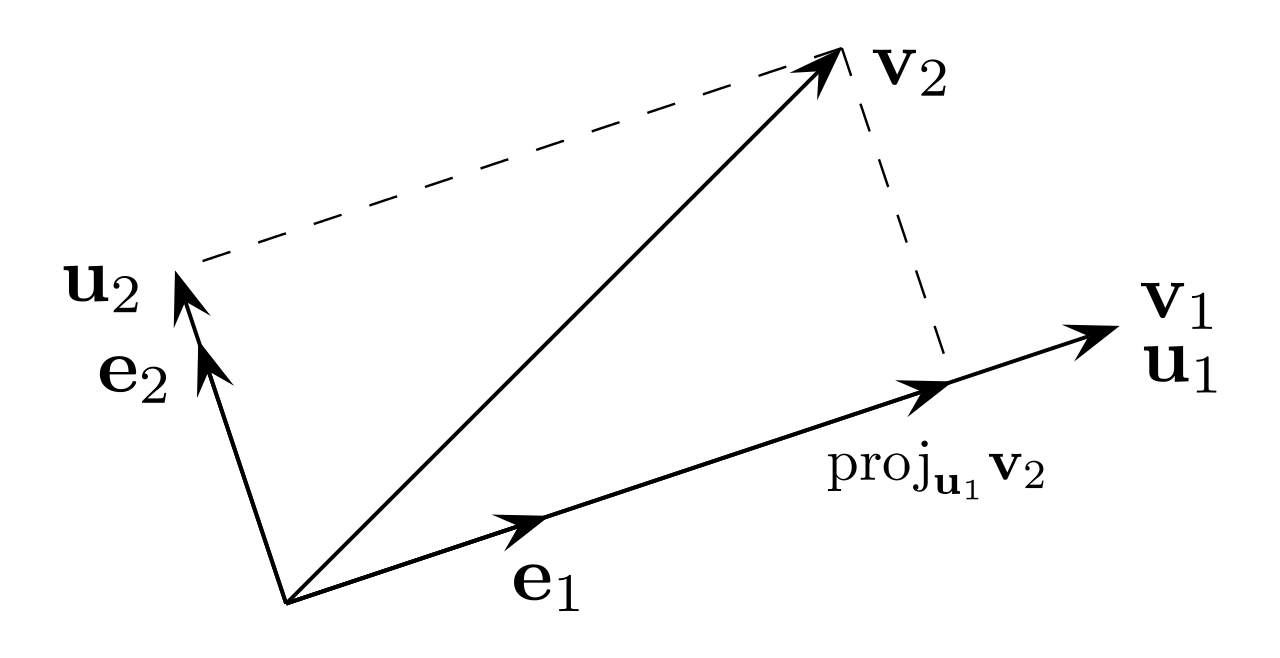
\includegraphics[scale=0.20]{15_6.png}

    \newpage

    \section{Liczby Stirlinga I i II rodzaju i ich interpretacja.}


    \begin{definition}
        \textbf{Liczby Stirlinga I rodzaju}.

        Dla dowolnego $n \geq 1$ mamy:
        \begin{enumerate}
            \item $c(0,0) = 1$
            \item $c(n,0) = c(0,n) = 0$
            \item $c(n,k) = c(n-1, k-1) + (n-1) * c(n-1, k)$
        \end{enumerate}
        W szczególności:
        \begin{enumerate}
            \item $c(n,n) = 1, c(n,1) = (n-1)!$
            \item $\sum^n_{k=0} c(n,k) = n!$
        \end{enumerate}

        \textbf{Interpretacja}: Przez $c(n,k)$ ($[^n_k]$) oznaczamy liczbę permutacji zbioru n-elementowego, które mają rozkład
        na dokładnie k cykli rozłącznych.
    \end{definition}

    \begin{definition}
        \textbf{Liczby Stirlinga II rodzaju}.

        Dla dowolnego $n \geq 1$ mamy:
        \begin{enumerate}
            \item $S(0,0) = 1$,
            \item $S(n,0) = S(0,n) = 0$,
            \item $S(n,k) = S(n-1, k-1) + k \times S(n-1, k)$.
        \end{enumerate}
        w szczególności  $S(n,n) = S(n,1) = 1$.\\

        \textbf{Interpretacja}: Przez $S(n,k)$ ($\{^n_k\}$) oznaczamy liczbę rozmieszczeń n rozróżnialnych kul na k nierozróżnialnych stosach w taki sposób,
        aby żaden stos nie był pusty.
    \end{definition}


    \newpage

    \section{Twierdzenia Eulera i Fermata; funkcja Eulera.}
    \begin{definition}
        \textbf{Funkcja Eulera (Tocjent)}

        Funkcja przypisująca każdej liczbie naturalnej liczbę liczb względnie pierwszych z nią i nie większych od niej.\newline $\sum_{m|n}^{} \varphi(m) = n$\newline

        \textbf{Własności}
        \begin{enumerate}
            \item $\varphi (n) \leq n - 1$  dla każdego $n>1$
            \item $\varphi (p) \leq p - 1$ dla każdego p będącego liczbą pierwszą
            \item $\varphi (mn) = \varphi (m)\varphi(n)$ jeśli NWD(m,n) = 1 (m i n względnie pierwsze)
            \item $\varphi(p^{k}) = p^{k-1} \cdot (p-1)$ jeśli p jest liczbą pierwszą
            \item $\varphi(n) = n
            \left (  1 - \frac{1}{p_1}\right)
            \left (  1 - \frac{1}{p_2}\right)
            \cdots
            \left (  1 - \frac{1}{p_n}\right)$
            gdzie $p_1, p_2, \dots, p_n$ są czynnikami pierwszymi liczby n
            \item jeżeli $n = \prod_{i=1}^{k} p_i^{k_i}$ jest rozkładem liczby n na czynniki pierwsze $\varphi (n) = \prod_{i=1}^{k} \varphi \left( p_i^{k_i} \right )$
        \end{enumerate}
    \end{definition}

    \begin{definition}
        \textbf{Małe Twierdzenie Fermata}

        Jeżeli p jest liczbą pierwszą, to dla dowolnej liczby całkowitej a, liczba $a^{p}-a$ jest podzielna przez p.\newline
        \begin{enumerate}
            \item $a^{p-a} \equiv 0 \pmod p$\newline
        \end{enumerate}

        Jeśli p jest liczbą pierwszą, a a jest taką liczbą całkowitą, że liczby a i p są względnie pierwsze to $a^{p-1} - 1$ dzieli się przez p.\newline

        \begin{enumerate}
            \item$a^{p-1} - 1 \equiv \pmod p$
            \item$a^{p-1} \equiv 1 \pmod p$
        \end{enumerate}

    \end{definition}

    \begin{definition}
        \textbf{Twierdzenie Eulera}

        Jeżeli $m \in \mathbb{Z_{+}}$ oraz $a \in \mathbb{Z}$ są liczbami względnie pierwszymi to m dzieli liczbę $a^{\varphi(m)} - 1$, gdzie $\varphi (m)$ oznacza wartość funkcji Eulera.

        \begin{enumerate}
            \item $a^{\varphi (m)} \equiv 1 \pmod m$\newline
        \end{enumerate}

    \end{definition}
    \newpage

    \section{Konfiguracje i t-konfiguracje kombinatoryczne.}

    \begin{definition}
        \textbf{Konfiuracją kombinatoryczną} $B$ o parametrach $(n,k,r)$ nazywamy rodzinę $k$-elementowych podzbiorów w $X$, jeżeli każdy element $x \in X$ występuje w dokładnie $r$ podbiorach. Zachodzą warunki:
        \begin{enumerate}
            \item $n = |X|$
            \item $|B_i|=k \quad \forall i=1, \dots, b$
            \item $n \cdot r = b \cdot k$ \quad gdzie b to liczba k-elementowych podzbiorów zbioru n-elementowego
        \end{enumerate}
    \end{definition}

    \begin{theorem}
        Istnieje konfiguracja kombinatoryczna $B$ o parametrach $(n, k, r)$ wtedy i tylko wtedy, gdy:
        \begin{enumerate}
            \item $k | n\cdot r$
            \item $\frac{n\cdot r}{k}\leq {n\choose k}$
        \end{enumerate}

    \end{theorem}

    \begin{definition}
        Niech $X$ dowolny zbiór, $|X| = n.$ $B$ rodzina $k-$ podzbiorów $X$ jest
        \textbf{t-konfiguracją kombinatoryczną} o parametrach $(n, k, r_t)$ wtw gdy dla
        każdego $t-$podzbioru $T \subset X$ liczba bloków z $B$ zawierających $T$ jest
        równa $r_t$.
    \end{definition}

    \begin{theorem}
        Jeśli $B$ jest $t$-konfiguracją kombinatoryczną, to
        $B$ jest $s$-konfiguracją kombinatoryczną dla $s = 1, 2,\dots$ $t-1$.
        Uwagi:
        \begin{enumerate}
            \item $r_{t-1}$ $= r_t \cdot \frac{n-t+1}{k-t+1}$
            \item Jeżeli $B$ jest $t-$konfiguracją o parametrach $(n,k,r_t)$, to dla $1 \leq s \leq (t-1)$
            \begin{align*}
                r_s = r_t \cdot \frac{(n-s)(n-s-1)\dots(n-t+1)}{(k-s)(k-s-1)\dots(k-t+1)}
            \end{align*}
            \item Jeśli $B$ jest $t$-konfiguracją o parametrach $(n,k,r_t)$, to
            \begin{align*}
                (k-s)(k-s-1)\dots(k-t+1)|r_t(n-s)(n-s-1)\dots(n-t+1) \\ dla\  0\leq s \leq (t-1)
            \end{align*}
            warunek 3. dla $t\geq 2$ jest konieczny dla istnienia $t$-konfiguracji, ale nie wystarczający
        \end{enumerate}
    \end{theorem}

    \newpage

    \section{Cykl Hamiltona, obwód Eulera, liczba chromatyczna - definicje i twierdzenia.}

    \subsection{Cykl Hamiltona}
    \begin{definition}
        \textbf{Ścieżka Hamiltona}. Ścieżką Hamiltona w grafie $G$ nazywamy ścieżkę, która przechodzi przez wszystkie
        wierzchołki $G$.
    \end{definition}

    \begin{definition}
        \textbf{Cykl Hamiltona}. Powiemy, że graf $G$ ma cykl Hamiltona, jeśli istnieje w nim cykl przechodzący przez
        wszystkie wierzchołki. Taki graf nazwyamy hamiltonowskim.
    \end{definition}

    \begin{theorem}
        Niech $G = (V, E)$ będzie grafem o $n \geq 3$ wierzchołkach. Jeśli dla dowolonych różnych, niesąsiednich
        wierzchołków $u, v \in V$ zachodzi warunek $d(u) + d(v) \geq n$, to G jest hamiltonowski.
    \end{theorem}

    \begin{theorem}
        Jeśli $G$ jest grafem o $n \geq 3$ wierzchołkach w którym minimalny stopień wierzchołka wynosi co najmniej
        $\frac{n}{2}$, to G jest hamiltonowski.
    \end{theorem}

    \begin{theorem}
        Niech $G = (V, E)$ będzie grafem o $n \geq 2$ wierzchołkach i takim, że $d(u) + d(v) \geq n-1$ dla dwóch dowolnych
        różnych, niesąsiednich wierzchołków $u, v \in V$. Wtedy G ma ścieżkę hamiltona.
    \end{theorem}

    \subsection{Obwód Eulera}
    \begin{definition}
        \textbf{Droga Eulera}. Drogą Eulera w grafie $G$ nazywamy drogę $v_1, v_2, \dots, v_m$, w której każda krawędź grafu G użyta
        jest dokładnie raz.
    \end{definition}
    \begin{definition}
        \textbf{Obwód Eulera}. Jeśli w grafie $G$ istnieje droga Eulera, w której pierwszy i ostatni wierzchołek są identyczne, to nazywamy ją
        obwodem Eulera. Graf ten nazywamy wtedy eulerowskim.
    \end{definition}

    \begin{theorem}
        Niech $G$ będzie grafem spójnym. Wówczas następujące warunki są równowaźne:
        \begin{enumerate}
            \item G jest grafem eurelowskim,
            \item stopień każdego wierzchołka w G jest parzysty.
        \end{enumerate}
    \end{theorem}

    \begin{theorem}
        Niech G będzie grafem spójnym. Wówczas G ma drogę Eulera $\Leftrightarrow$ w G są dokładnie zero lub dwa wierzchołki
        stopnia nieparzystego.
    \end{theorem}

    \subsection{Liczba chromatyczna}
    \begin{definition}
        \textbf{Kolorowanie wierchołkowe}. Kolorowaniem wierzchołkowym grafu $G = (V, E)$ przy użyciu (co najwyżej) $k$
        kolorów nazywamy funkcję $c: V \rightarrow \{1, \dots, k\}$ spełniającą warunek
        $c(u) \neq c(v) ~~ \forall u, v \in V : uv \in E$.
    \end{definition}

    \begin{definition}
        \textbf{Liczba chromatyczna}. Liczbą chromatyczną grafu G nazywamy najmniejszą liczbę $k \in \mathbb{N}$, dla
        której istnieje kolorwanie wierzchołkowe G przy użyciu k kolorów. Oznaczamy $\chi(G)$.
        \begin{enumerate}
            \item $\chi(G) = 1 \Leftrightarrow |E(G)| = 0$
            \item $\chi(T) = 2$ dla każdego drzewa T o przynajmniej dwóch wierzchołkach
            \item $\chi(C_{2k}) = 2, \chi(C_{2k+1}) = 3$
            \item $\chi(K_n) = n$
        \end{enumerate}
    \end{definition}

    \begin{theorem}
        Niech G będzie dowolnym grafem. Wtedy $\chi(G) \leq d_{\max}(G) + 1$.
    \end{theorem}

    \begin{theorem}
        Niech G będzie grafem spójnym. Wówczas $\chi(G) \leq d_{\max}(G)$, o ile G nie jest grafem pełnym ani cyklem o
        nieparzystej liczbie wierzchołków.
    \end{theorem}

    \newpage

    \section{Algorytm Forda-Fulkersona wyznaczania maksymalnego przepływu.}

    \begin{definition}
        \textbf{Siecią przepływową} nazywamy zestaw $(V, \vec{E}, s, t, c)$, gdzie $(V, \vec{E})$ jest grafem
        skierowanym wraz z wyróżnionymi wierzchołkami $s$ - \textbf{źródłem} i $t$ - \textbf{ujściem} oraz
        \textbf{funkcją pojemności krawędzi} $c: ~ \vec{E} \rightarrow \mathbb{R}$.
    \end{definition}

    \begin{definition}
        \textbf{Przepływem} w sieci $(V, \vec{E}, s, t, c)$ nazywamy funkcję $f: \vec{E} \rightarrow \mathbb{R}$
        spełniającą następujące warunki:
        \begin{enumerate}
            \item $f(\vec{uv}) \leq c(\vec{uv})$  dla każdej krawędzi $\vec{uv} \in \vec{E}$,
            \item dla każdego ustalonego $v \in V \backslash \{s, t\}:$
            \begin{align*}
                \sum_{\vec{uv} \in \vec{E}} ~ f(\vec{uv}) ~~ = ~~ \sum_{\vec{vw} \in \vec{E}} ~ f(\vec{vw}).
            \end{align*}
        \end{enumerate}
        Liczbę $|f| =  \sum_{\vec{su}  \in \vec{E}} f(\vec{su}) = \sum_{\vec{wt} \in \vec{E}} f(\vec{wt})$ nazywamy
        \textbf{wartością przepływu} f.\\

        Przepływ f nazywamy \textbf{maksymalnym}, jeśli jego wartość jest największa spośród wszystkich przepływów w
        danej sieci.
    \end{definition}

    \begin{definition}
        Niech $(V, \vec{E}, s, t, c)$ będzie siecią przepływową oraz $f$ pewnym przepływem tej sieci. \textbf{Siecią rezydualną}
        nazywamy sieć $G_f = (V, E_f, s, t, c_f)$, gdzie $E_f = \vec{E} \cup \{\vec{vu}: \vec{uv} \in \vec{E}\}$ z funkcją
        pojemności określoną wzorem:
        \begin{align*}
            c_f(\vec{uv}) = c(\vec{uv}) - f(\vec{uv}) ~~ \text{dla} ~ \vec{uv} \in  \vec{E} ~  \text{t. że} ~ c(\vec{uv}) > 0
        \end{align*}
        \begin{align*}
            c_f(\vec{uv}) = f(\vec{uv}) ~~ \text{dla} ~ \vec{uv} \notin  \vec{E} ~  \text{t. że} ~ \vec{vu} \in \vec{E} \text{i} f(\vec{uv}) > 0
        \end{align*}
        oraz $c_f(\vec{uv}) = 0$ w pozostałych przypadkach.
    \end{definition}

    \begin{definition}
        \textbf{Ścieżką rozszerzającą} dla przepływu f nazywamy dowolną ścieżkę (skierowaną) $v_0 \rightarrow v_1 \rightarrow \cdots \rightarrow v_k$
        w sieci rezydualnej $G_f$ łączącą wierzchołki $v_0 = s$ i $v_k = t$, w której $c_f(\vec{v_i v_{i+1}}) > 0$ dla
        każdego $i = 0, \cdots, k-1$.
    \end{definition}

    \begin{theorem}
        \textbf{Algorytm Forda-Fulkersona}. W celu znalezienia maksymalnego przepływu $f$ w sieci przepływowej
        $(V, \vec{E}, s, t, c)$:
        \begin{enumerate}
            \item przyjmujemy początkowo dowolny (np. zerowy) przepływ $f$,
            \item budujemy sieć rezydualną $G_f$,
            \item dopóki w $G_f$ istnieje ścieżka rozszerzająca $P = v_0 \rightarrow v_1 \rightarrow \cdots \rightarrow v_k$
            określamy $c_p = min_{i = 0, \cdots, k-1} c_f(\vec{v_i v_{i+1}})$, a następnie zwiększamy o $c_p$ wartość
            przepływu $f$ na krawędziach $\vec{v_i v_{i+1}}$ tej ścieżki i uaktualniamy wartości funkcji $c_f$ sieci
            rezydualnej.
        \end{enumerate}
    \end{theorem}

    \begin{definition}
        \textbf{Przekrojem} w sieci przepływowej $(V, \vec{E}, s, t, c)$ nazywamy parę zbiorów $(S, T)$ spełniającą
        warunki:
        \begin{enumerate}
            \item $S \cup T = V$,
            \item $S \cap T = \emptyset$,
            \item $s \in S, t \in T$.
        \end{enumerate}

        \textbf{Pojemnością} przekroju $(S,T)$ nazywamy liczbę
        \begin{align*}
            c(S, T) = \sum_{(u,v) \in \vec{E} \cap (S \times T)} c(\vec{uv}).
        \end{align*}
    \end{definition}

    \begin{theorem}
        Niech $(V, \vec{E}, s, t, c)$ będzie siecią przepływową. Wówczas \textbf{maksymalna wartość przepływu jest
        jest równa minimalnej pojemności} przekroju w tej sieci.
    \end{theorem}

    \newpage

    \section{Rozwiązywanie równań rekurencyjnych przy użyciu funkcji tworzących (generujących) oraz przy użyciu
    równania charakterystycznego.}

    \begin{definition}
        \textbf{Liniowym równaniem rekurencyjnym rzędu r} (o stałych współczynnikach) nazywamy równanie postaci:
        \begin{align*}
            x_{n+r} = c_1 x_{n+r-1} +  \cdots + c_r x_n + f(n)
        \end{align*}
        w którym $c_i  \in \mathbb{R}, c_r \neq 0$  oraz $f:  \mathbb{N} \rightarrow \mathbb{R}$ jest dowolną funkcją.
        Jeśli funkcja f jest stale równa zero, to powyższe równanie nazywamy \textbf{jednorodnym}.
    \end{definition}

    \begin{definition}
        \textbf{Rozwiązaniem szczególnym} równania nazywamy dowolny ciąg $(x_n)$ spełniający zależność rekurencyjną.
        Dla każdego równania jednorodnego rozwiązanie szczególnym jest ciąg stały równy zero.

        \textbf{Rozwiązaniem ogólnym} równania nazywamy wzór ogólny (zależny od pewnych parametrów) pozwalający
        wyznaczyć wszystkie rozwiązania szczególne.
    \end{definition}

    \subsection{Funkcje tworzące.}
    \begin{definition}
        \textbf{Funkcją tworzącą} (generujacą) ciągu $(a_n)$ nazywamy szereg
        \begin{align*}
            \sum_{n=0}^{\infty} a_n x^n.
        \end{align*}
        Jest to tylko inny zapis ciągu (wyraz $a_n$ to współczynnik przy $x^n$) - nie interesują nas kwestie zbieżności,
        podstawiania wartości za x, ciągłości/różniczkowalności funkcji określonej takim szeregiem itd.

        Jeżeli jednak funkcja tworząca pewnego ciągu "wygląda" jak zbieżny szereg określający funkcję znaną z analizy
        to możemy używać skróconego zapisu, np. $\sum_{n=0}^{\infty} \frac{1}{n!} x^n = e^x$.
    \end{definition}

    \begin{theorem}
        \textbf{Operacje na funkcjach tworzących}.
        \begin{enumerate}
            \item Funkcje tworzące można \textbf{dodawać,odejmować i mnożyć przez liczbę} - odpowiadają temu operacje
            dodawania, odejmowania i mnożenia przez liczbę wyrazów ciągu.
            \item \textbf{Mnożeniu dwóch funkcji tworzących} odpowiada operacja "splotu", tzn. jeśli
            $A(x) =  \sum_{n=0}^{\infty} a_n x^n$ i $B(x) = \sum_{n=0}^{\infty} b_n x^n$, to
            $A(x) * B(x) = \sum_{n=0}^{\infty} c_n x^n$, gdzie $c_n = \sum_{k=0}^n a_k b_{n-k}$.
            \item Jeśli funkcja tworząca A(x) ma "element odwrotny", tzn. taką funkcję tworzącą B(x) dla której
            $A(x) * B(x) = 1$, to mówimy że A(x) jest \textbf{odwracalna} i piszemy $\frac{1}{A(x)} = B(x)$.
            \item \textbf{Mnożeniu funkcji} tworzącej \textbf{przez x} odpowiada przesunięcie ciągu (dopisanie na początek
            wyrazu zerowego). Operajcją odwrotną jest odjęcie wyrazu zerowego i podzielenie przez x.
            \item Funkcje tworzące można \textbf{różniczkować} według wzoru:
            \begin{align*}
                (\sum_{n=0}^{\infty} a_n x^n)' = \sum_{n=1}^{\infty} n a_n x^{n-1} = \sum_{n=0}^{\infty} (n+1) a_{n+1} x^n
            \end{align*}
            \item Zachodzą wzory na \textbf{pochodne} znane z analizy, np. $(A(x) * B(x))' = A'(x)B(x) + A(x)B'(x)$.
            \item Operacja \textbf{"całkowania"} (odwrotna do różniczkowania):
            \begin{align*}
                \int (\sum_{n=0}^{\infty} a_n x^n) = \sum_{n=0}^{\infty} \frac{a_n}{n+1} x^{n+1} = \sum_{n=0}^{\infty} \frac{a_n - 1}{n} x^n
            \end{align*}
            Wyraz $a_n$ można "odzyskać" z funkcji tworzącej A(x) wykonując jej n-krotne różniczkowanie.
        \end{enumerate}
    \end{theorem}

    \begin{theorem}
        Dla dowolnej liczby naturalnej $m \geq 1$ zachodzi wzór:
        \begin{align*}
            \frac{1}{(1-x)^m} ~ = ~ \sum_{n=0}^{\infty} \binom{n+m-1}{n} x^n.
        \end{align*}

        Dla dowolnego $\alpha \in \mathbb{R}$ oraz $|x| < 1$ zachodzi wzór:
        \begin{align*}
            (1+x)^{\alpha} ~ = ~ \sum_{n=0}^{\infty} \binom{\alpha}{n} x^n
        \end{align*}
    \end{theorem}

    \subsection{Równanie charakterystyczne.}
    \begin{definition}
        \textbf{Równanie charakterystyczne} równania rekurencyjnego. Weźmy równanie rekurencyjne jednorodne
        \begin{align*}
            a_n = A a_{n-1} + B a_{n-2}
        \end{align*}
        gdzie dane są współczynniki A, B. Załóżmy, że ma ono rozwiązanie postaci $a_n = t^n$. Podstawiając otrzymujemy:
        \begin{align*}
            t^n = A t^{n-1} + B t^{n-2}.
        \end{align*}
        Dzielimy obie strony przez $t^{n-2}$:
        \begin{align*}
            t^2 = A t^1 + B
        \end{align*}
        \begin{align*}
            t^2 - A t^1 - B = 0.
        \end{align*}
        Równanie to nazywamy równaniem charakterystycznym równania rekurencyjnego. W tym przypadku jest to równanie kwadratowe.

        Jeżeli nie ma ono pierwiastków podwójnych, wówczas:
        \begin{align*}
            a_n = C r_1^n + D r_2^n.
        \end{align*}
        Jeżeli ma pierwiastki podwójne, to:
        \begin{align*}
            a_n = (C + Dn) r_1^n.
        \end{align*}
        C i D są dowolnymi stałymi a $r_{1}$ i $r_{2}$ są pierwiastkami równania charakterystycznego. Jeżeli dane jest
        $a_{1}$ i $a_{2}$ wówczas można łatwo ułożyć układ równań i otrzymać ich wartość.
    \end{definition}

    \newpage

    \section{Ciąg i granica ciągu liczbowego, granica funkcji.}

    \subsection{Ciągi.}

    \begin{definition}
        \textbf{Ciąg liczbowy}. Ciągiem liczbowym nazywamy funkcję $\mathbb{N} \rightarrow \mathbb{R}$. Wartość tej
        funkcji dla liczby naturalnej $n$ nazywamy $n$-tym wyrazem ciągu i oznaczamy przez $a_n$, $b_n$ itp. Ciągi o
        takich wyrazachoznaczamy odpowiednio przez $(a_n)$, $(b_n)$  itp. Zbiór wyrazów ciągu $(a_n)$, tj.
        $\{a_n : n  \in \mathbb{N}\}$ oznaczamy krótko przez  $\{a_n\}$.
    \end{definition}

    \begin{definition}
        \textbf{Granica właściwa ciągu}. Ciąg $(a_n)$ jest zbieżny do granicy właściwej $a \in \mathbb{R}$, co zapisujemy:
        \begin{align*}
            lim_{n  \rightarrow \infty} ~ a_n = a
        \end{align*}
        wtedy i tylko wtedy, gdy
        \begin{align*}
            \forall \varepsilon > 0 ~~ \exists  n_0 \in \mathbb{N} ~~ \forall n \in \mathbb{N} ~~~ [(n > n_0) \Rightarrow (|a_n - a| < \varepsilon)]
        \end{align*}
    \end{definition}

    \begin{definition}
        \textbf{Granice niewłaściwe ciągu}.

        Ciąg $(a_n)$ jest zbieżny do granicy niewłaściwej $\infty$, co zapisujemy:
        \begin{align*}
            lim_{n \rightarrow \infty} ~ a_n = \infty
        \end{align*}
        wtedy i tylko wtedy, gdy:
        \begin{align*}
            \forall \varepsilon > 0 ~~ \exists  n_0 \in \mathbb{N} ~~ \forall n \in \mathbb{N} ~~~ [(n > n_0) \Rightarrow (a_n > \varepsilon)]
        \end{align*}

        Ciąg $(a_n)$ jest zbieżny do granicy niewłaściwej $-\infty$, co zapisujemy:
        \begin{align*}
            lim_{n \rightarrow \infty} a_n = -\infty
        \end{align*}
        wtedy i tylko wtedy, gdy:
        \begin{align*}
            \forall \varepsilon < 0 ~~ \exists  n_0 \in \mathbb{N} ~~ \forall n \in \mathbb{N} ~~~ [(n > n_0) \Rightarrow (a_n < \varepsilon)]
        \end{align*}
    \end{definition}

    \begin{theorem}
        \textbf{O ograniczoności ciągu zbieżnego}. Jeśli ciąg jest zbieżny do granicy właściwej, to jest ograniczony.
    \end{theorem}

    \begin{theorem}
        \textbf{O równoważności granic.}
        \begin{align*}
            lim_{n \rightarrow \infty} ~ a_n = 0 ~~ \Leftrightarrow ~~ lim_{n \rightarrow \infty} ~ |a_n| = 0.
        \end{align*}
    \end{theorem}

    \begin{theorem}
        \textbf{O dwóch ciągach}. Jeśli ciągi $(a_n)$, $(b_n)$ spełniają warunki:
        \begin{enumerate}
            \item $a_n \leq b_n ~~~ \forall n \geq n_0$
            \item $lim_{n \rightarrow \infty} a_n = \infty$
        \end{enumerate}
        to
        \begin{align*}
            lim_{n \rightarrow \infty} ~ b_n = \infty.
        \end{align*}

        Prawdziwe jest także analogiczne twierdzenie dla ciągów zbieżnych do granicy niewłaściwej $-\infty$.
    \end{theorem}

    \begin{theorem}
        \textbf{O trzech ciągach}. Jeśli ciągi $(a_n)$, $(b_n)$, $(c_n)$ spełniają warunki:
        \begin{enumerate}
            \item $a_n \leq b_n \leq c_n ~~~ \forall n \geq n_0$
            \item $lim_{n  \rightarrow \infty} a_n = lim_{n \rightarrow \infty} c_n = b$
        \end{enumerate}
        to
        \begin{align*}
            lim_{n \rightarrow \infty} ~ b_n = b.
        \end{align*}
    \end{theorem}

    \begin{theorem}
        \textbf{O ciągu monotonicznym i ograniczonym}. Jeżeli ciąg $(a_n)$ jest niemalejący dla $n \geq n_0$ oraz
        ograniczony z góry, to jest zbieżny do granicy właściwej $\sup\{a_n : n \geq n_0\}$.

        Prawdziwe jest także analogiczne twierdzenie dla ciągu nierosnącego i ograniczonego z dołu.
    \end{theorem}

    \subsection{Funkcje.}

    \begin{definition}
        \textbf{Heinego granicy właściwej funkcji w punkcie}. Niech $x_0 \in \mathbb{R}$ oraz niech funkcja $f$ będzie
        określona przynajmniej na sąsiedztwie $S(x_0)$. Liczba $g$ jest granicą właściwą funkcji $f$ w punkcie $x_0$, co
        zapisujemy
        \begin{align*}
            lim_{x \rightarrow x_0} ~ f(x) = g
        \end{align*}
        wtedy i tylko wtedy, gdy
        \begin{align*}
            \forall_{(x_n): ~ \{x_n\} \subset S(x_0)} ~~ [(lim_{n \rightarrow \infty} x_n = x_0) \Rightarrow (lim_{n \rightarrow \infty} f(x_n) = g)].
        \end{align*}
    \end{definition}

    \begin{definition}
        \textbf{Cauchy'ego granicy właściwej funkcji w punkcie}. Niech $x_0 \in \mathbb{R}$ oraz niech funkcja $f$ będzie
        określona przynajmniej na sąsiedztwie $S(x_0)$. Liczba $g$ jest granicą właściwą funkcji $f$ w punkcie  $x_0$,
        co zapisujemy
        \begin{align*}
            lim_{x \rightarrow x_0} ~ f(x)  = g
        \end{align*}
        wtedy i tylko wtedy, gdy
        \begin{align*}
            \forall \varepsilon > 0 ~~ \exists \delta > 0 ~~ \forall  x \in S(x_0)  ~~~ [(|x - x_0| <  \delta) \Rightarrow (|f(x) - g| < \varepsilon)].
        \end{align*}
        \hfill \\

        Funkcja $f$ ma granicę niewłaściwą $\infty$ w punkcie $x_0$ wtedy i tylko wtedy, gdy
        \begin{align*}
            \forall \varepsilon > 0 ~~ \exists \delta > 0 ~~ \forall  x \in S(x_0)  ~~~ [(|x - x_0| <  \delta) \Rightarrow (f(x) > \varepsilon)].
        \end{align*}

    \end{definition}

    \begin{theorem}
        \textbf{O nieistnieniu granicy funkcji w punkcie}. Jeśli istnieją ciągi $(x'_n)$, $(x''_n)$ spełniające warunki:
        \begin{enumerate}
            \item $lim_{n \rightarrow \infty} x'_n = x_0$, przy czym $x'_n \neq x_0 ~~ \forall n \in \mathbb{N}$
            oraz $lim_{n \rightarrow \infty}  ~ f(x'_n) = g'$,
            \item $lim_{n \rightarrow \infty} x''_n = x_0$, przy czym $x''_n \neq x_0 ~~ \forall n \in \mathbb{N}$
            oraz $lim_{n \rightarrow \infty}  ~ f(x''_n) = g''$,
            \item $g' \neq g''$,
        \end{enumerate}
        to granica $lim_{x \rightarrow x_0} ~ f(x)$ nie istnieje (właściwa ani niewłaściwa).
    \end{theorem}

    \begin{theorem}
        \textbf{Warunek konieczny i wystarczajacy istnienia granicy}. Funckja $f$ ma w punkcie $x_0$ granicę
        właściwą (niewłaściwą) wtedy i tylko wtedy, gdy
        \begin{align*}
            lim_{x \rightarrow x^{-}_0}  ~ f(x) ~ = ~ lim_{x \rightarrow x^{+}_0}  ~ f(x)
        \end{align*}
        Wspólna wartość granic jednostronnych jest wtedy granicą funkcji.
    \end{theorem}

    \begin{theorem}
        \textbf{O niesitnieniu granicy funkcji w nieskończoności}. Jeżeli istnieją ciągi $(x'_n)$, $(x''_n)$
        spełniające warunki:
        \begin{enumerate}
            \item $lim_{n \rightarrow \infty} ~ x'_n = \infty $ oraz $ lim_{n \rightarrow \infty} ~ f(x'_n) = g'$,
            \item $lim_{n \rightarrow \infty} ~ x''_n = \infty $ oraz $ lim_{n \rightarrow \infty} ~ f(x''_n) = g''$,
            \item $g' \neq g''$,
        \end{enumerate}
        to nie istnieeje granica $lim_{x \rightarrow x_0} ~ f(x)$ (właściwa ani niewłaściwa).
    \end{theorem}

    \begin{theorem}
        \textbf{O dwóch funkcjach}. Jeśli funkcje $f$ i $g$ spełniają warunki:
        \begin{enumerate}
            \item $f(x) \leq g(x) ~~ \forall x \in S(x_0)$,
            \item $lim_{x \rightarrow x_0} ~ f(x) = \infty$,
        \end{enumerate}
        to
        \begin{align*}
            lim_{x \infty x_0} ~ g(x) = \infty.
        \end{align*}
    \end{theorem}

    \begin{theorem}
        \textbf{Granice specjalne}
        \setlength{\jot}{10pt}
        \begin{align*}
            &\lim_{x \to +\infty} a^{x} x^{\alpha} \stackrel{[0 \cdot \infty]}{=}  \text{0 dla a} \in (0, 1), \alpha \geq 0 \\
            &\lim_{x \to 0} \frac{\sin{x}}{x} \stackrel{[\frac{0}{0}]}{=} \text{1 oraz}    \lim_{x \to 0} \frac{\arcsin{x}}{x} \stackrel{[\frac{0}{0}]}{=} 1\\
            &\lim_{x \to 0} (1 + x)^{\frac{1}{x}} \stackrel{1^{\infty}}{=} \text{e oraz}   \lim_{x \to \infty} (1 + x)^{\frac{1}{x}} \stackrel{\infty^{0}}{=} 1 \\
            &\lim_{x \to 0} \frac{a^x -1}{x} \stackrel{[\frac{0}{0}]}{=} \ln{a} \text{ dla a $>$ 0, w szczególności } \lim_{x \to 0} \frac{e^x -1}{x} \stackrel{[\frac{0}{0}]}{=} 1 \\
            &\lim_{x \to 0} \frac{\log_{a}(1 + x)}{x} \stackrel{[\frac{0}{0}]}{=} \frac{1}{\ln{a}} \text{, w szczególności } \lim_{x \to 0} \frac{\ln(1 + x)}{x} \stackrel{[\frac{0}{0}]}{=} 1 \\
            &\lim_{x \to \pm \infty} (1 + \frac{a}{x})^{x} \stackrel{[1^{\infty}]}{=} e^{a} \text{, dla a} \in \mathbb{R} \\
            &\lim_{x \to 0} \frac{(1 + x)^a - 1}{x} \stackrel{[\frac{0}{0}]}{=} \text{a, dla a} \in \mathbb{R}
        \end{align*}
    \end{theorem}

    \begin{theorem}
        \textbf{Reguła de L'Hostpiala}. Jeżeli funkcja $f$ i  $g$ spełniają warunki:
        \begin{enumerate}
            \item $lim_{x \rightarrow x_0} f(x) = lim_{x \rightarrow x_0} g(x) = 0 ~~ (\infty)$, przy czym $g(x) \neq 0$ dla $x \in S(x_0)$
            \item istnieje granica $lim_{x \rightarrow x_0} \frac{f'(x)}{g'(x)}$ (właściwa lub niewłaściwa),
        \end{enumerate}
        to
        \begin{align*}
            lim_{x \rightarrow x_0} \frac{f(x)}{g(x)} = lim_{x \rightarrow x_0} \frac{f'(x)}{g'(x)}
        \end{align*}
    \end{theorem}

    \newpage

    \section{Ciągłość i pochodna funkcji. Definicja i podstawowe twierdzenia.}

    \subsection{Ciągłość.}

    \begin{definition}
        \textbf{Funkcja ciągła w punkcie}. Niech $x_0 \in \mathbb{R}$ oraz niech funkcja $f$ będzie określona przynajmniej
        na otoczeniu $O(x_0)$. Funkcja $f$ jest ciągła w ounkcie $x_0$ wtedy i tylko wtedy, gdy
        \begin{align*}
            lim_{x \rightarrow x_0} ~ f(x) = f(x_0).
        \end{align*}
        \hfill \\

        \textbf{Funkcja jest ciągła na zbiorze}, jeżeli jest ciągła w każdym punkcie tego zbioru.
    \end{definition}

    \begin{theorem}
        \textbf{Warunek konieczny i wystarczający ciągłości funkcji}. Funckja jest ciągła w punkcie wtedy i tylko wtedy,
        gdy jest w tym punkcie ciągła lewostronnie i prawostronnie.
    \end{theorem}

    \begin{definition}
        \textbf{Nieciągłość funkcji}. Niech $x_0 \in \mathbb{R}$ oraz niech funkcja $f$ będzie określona przynajmniej
        na otoczeniu $O(x_0)$. Funkcja $f$ jest nieciągła w punkcie $x_0$ wtedy i tylko wtedy, gdy nie istnieje
        granica $lim_{x \rightarrow x_0} ~ f(x)$ albo gdy $lim_{x \rightarrow x_0} ~ f(x) \neq f(x_0)$.
        \hfill \\

        \textbf{Nieciągłość pierwszego rodzaju}. Jeżeli istnieją granice skończone $lim_{x \rightarrow x^{-}_0 ~ f(x)}$,
        $lim_{x \rightarrow x^{+}_0} ~ f(x)$ oraz
        \begin{align*}
            lim_{x \rightarrow x^{-}_0} ~ f(x) \neq  f(x_0) ~~~ \text{lub} ~~~ lim_{x \rightarrow x^{+}_0} ~ f(x) \neq f(x_0).
        \end{align*}
        Mówimy, że funkcja $f$ ma w punkcie $x_0$ nieciągłość pierwszego rodzaju typu "skok", jeżeli spełnia warunek
        \begin{align*}
            lim_{x \rightarrow x^{-}_0} ~ f(x) ~ \neq ~ lim_{x \rightarrow x^{+}_0} ~ f(x).
        \end{align*}
        Mówi, że funkcja $f$ ma w punkcie $x_0$ nieciągłość pierwszego rodzaju typu "luka", jeżeli spełnia warunek
        \begin{align*}
            lim_{x \rightarrow x^{-}_0} ~ f(x) ~ = ~ lim_{x \rightarrow x^{+}_0} ~ f(x) ~ \neq ~ f(x_0).
        \end{align*}
        \hfill \\

        \textbf{Nieciągłość drugiego rodzaju}. Jeżeli co najmniej jedna z granic
        \begin{align*}
            lim_{x \rightarrow x^{-}_0} ~ f(x), ~~ lim_{x \rightarrow x^{+}_0} ~ f(x)
        \end{align*}
        nie istnieje lub jest niewłaściwa.
    \end{definition}

    \begin{theorem}
        \textbf{Weierstrassa o ograniczoności funkcji ciągłej}. Jeżeli funkcja jest ciągła na przedziale domkniętym
        i ograniczonym, to jest na nim ograniczona.
    \end{theorem}

    \begin{theorem}
        \textbf{Weierstrassa o osiąganiu kresów}. Jeżeli funkcja $f$ jest ciągła na przedziale domkniętym $[a, b]$,to
        \begin{align*}
            \exists c \in [a,b] ~~ f(c) = ~ inf_{x \in [a,b]} ~ f(x) ~~ \text{oraz} ~~ \exists d \in [a,b] ~~ f(d) = ~ sup_{x \in [a,b]} ~ f(x)
        \end{align*}
    \end{theorem}

    \begin{theorem}
        \textbf{Darboux o przyjmowaniu wartości pośrednich}. Jeżeli funkcja $f$ jest ciągła na przedziale $[a,b]$ oraz
        spełnia warunek $f(a) < f(b)$, to
        \begin{align*}
            \forall w \in (f(a), f(b)) ~ \exists c \in (a,b) ~~ f(c) = w.
        \end{align*}
    \end{theorem}


    \subsection{Pochodna.}

    \begin{definition}
        \textbf{Iloraz różnicowy}. Niech  $x_0 \in \mathbb{R}$ oraz niech funkcja $f$ będzie określona przynajmniej
        na otoczeniu $O(x_0, r)$, gdzie $r > 0$. Ilorazem różnicowym funkcji $f$ w punkcie $x_0$  odpowiadającym przyrostowi
        $\Delta x$, gdzie $0 < |\Delta x| < r$, zmiennej niezależnej nazywamy liczbę
        \begin{align*}
            \frac{\Delta f}{\Delta x} \stackrel{def}{=} \frac{f(x_0 + \Delta x) - f(x_0)}{\Delta x}
        \end{align*}
    \end{definition}

    \begin{definition}
        \textbf{Pochodna właściwa funkcji}. Niech $x_0 \in \mathbb{R}$ oraz niech funkcja $f$ będzie określona przynajmniej
        na otoczeniu $O(x_0)$. Pochodną właściwą funkcji $f$ w punkcie $x_0$ nazywamy granicę właściwą
        \begin{align*}
            f'(x_0) ~ \stackrel{def}{=} ~ lim_{x \rightarrow x_0} ~ \frac{f(x) - f(x_0)}{x - x_0}
        \end{align*}

        Inaczej mówiąc pochodna funkcji $f$ jest granicą ilorazu różnicowego gdy $\Delta x \rightarrow 0$. Mamy zatem
        \begin{align*}
            f'(x_0) ~ \stackrel{def}{=} ~ lim_{\Delta x \rightarrow 0} ~ \frac{f(x_0 + \Delta x) - f(x_0)}{\Delta x}
        \end{align*}
    \end{definition}

    \begin{theorem}
        \textbf{Warunek konieczny istnienia pochodnej właściwej funkcji}. Jeżeli funkcja ma pochodną właściwą w punkcie,
        to jest ciągła w tym punkcie. Implikacja odwrotna nie jest prawdziwa.
    \end{theorem}

    \begin{definition}
        \textbf{Pochodne jednostronne właściwe funkcji}. Niech $x_0 \in \mathbb{R}$ oraz niech funkcja $f$ będzie
        określona przynajmniej na otoczeniu  $O(x^{-}_0)$. Pochodną lewostronną właściwą funkcji $f$ w punkcie $x_0$
        nazywamy granicę właściwą
        \begin{align*}
            f'_{-}(x_0) ~ \stackrel{def}{=} ~ lim_{x \rightarrow x^{-}_0} ~ \frac{f(x) - f(x_0)}{x - x_0}
        \end{align*}
        Analogicznie definiujemy $f'_{+}(x_0)$.\\

        Jeżeli funkcja ma w punkcie pochodną lewostronną (prawostronną) właściwą, to jest w nim ciągła lewostronnie
        (prawostronnie).
    \end{definition}

    \begin{definition}
        \textbf{Pochodna funkcji na zbiorze}. Funkcja ma pochodną właściwą na zbiorze wtedy i tylko wtedy, gdy ma pochodną
        właściwą w każdym punkcie tego zbioru.
    \end{definition}

    \begin{definition}
        \textbf{Pochodna niewłaściwa funkcji}. Niech $f$ będzie funkcją ciągłą w punkcie $x_0 \in \mathbb{R}$. Funkcja
        $f$ ma w punkcie $x_0$ pochodną niewłaściwą wtedy i tylko wtedy, gdy
        \begin{align*}
            lim_{x \rightarrow  x_0} ~ \frac{f(x) - f(x_0)}{x - x_0} = \infty ~~ \text{albo} ~~ lim_{x  \rightarrow x_0} ~ \frac{f(x) - f(x_0)}{x - x_0} = -\infty
        \end{align*}
        Podobnie definiujemy pochodne niewłaściwe jednostronne.
    \end{definition}

    \begin{theorem}
        \textbf{Zastosowanie różniczki do obliczeń przybliżonych}. Jeżeli funkcja $f$ ma pochodną właściwą w punkcie
        $x_0$, to
        \begin{align*}
            f(x_0 + \Delta x) \approx f(x_0) + f'(x_0)\Delta x
        \end{align*}
        Przy czym błąd, jaki popełniamy zastępując przyrost funkcji
        \begin{align*}
            \Delta f = f(x_0 \Delta x) - f(x_0)
        \end{align*}
        jej różniczką $df = f'(x_0)\Delta x$, dąży szybciej do zera niż przyrost zmiennej niezależnej $\Delta x$, tzn.
        \begin{align*}
            lim_{\Delta  x  \rightarrow 0} \frac{\Delta f - df}{\Delta  x} = 0.
        \end{align*}
    \end{theorem}

    \begin{theorem}
        \textbf{Rolle'a}. Jeśli funkcja $f$ spełnia warunki:
        \begin{enumerate}
            \item jest ciągła na $[a,b]$
            \item ma pochodną właściwą lub niewłaściwą na $(a,b)$,
            \item $f(a) = f(b)$,
        \end{enumerate}
        to istnieje punkt $c \in (a,b)$ taki, że:
        \begin{align*}
            f'(c) = 0.
        \end{align*}
    \end{theorem}

    \begin{theorem}
        \textbf{Lagrange'a}. Jeżeli funkcja $f$ spełnia warunki:
        \begin{enumerate}
            \item jest ciągła na $[a,b]$,
            \item ma pochodną właściwą lub niewłaściwą na $(a,b)$,
        \end{enumerate}
        to istnieje punkt $c \in (a,b)$ taki, że
        \begin{align*}
            f'(c) = \frac{f(b)-f(a)}{b-a}
        \end{align*}
    \end{theorem}

    \newpage

    \section{Ekstrema funkcji jednej zmiennej. Definicje i twierdzenia.}

    \begin{definition}
        \textbf{Minimum lokalne funkcji}. Funkcja $f$ ma w punkcie $x_0 \in \mathbb{R}$ minimum lokalne, jeżeli:
        \begin{align*}
            \exists \delta > 0 ~ \forall x \in S(x_0, \delta) ~~ f(x) \geq f(x_0).
        \end{align*}
        Analogicznie definiujemy \textbf{maksimum lokalne}.\\

        \textbf{Minimum lokalne jest właściwe}, jeżeli:
        \begin{align*}
            \exists \delta > 0 ~ \forall x \in S(x_0, \delta) ~~ f(x) > f(x_0).
        \end{align*}
        Analogicznie definiujemy \textbf{maksimum lokalne właściwe}.\\
    \end{definition}

    \begin{theorem}
        \textbf{Fermata, warunek konieczny istnienia ekstremum}. Jeżeli funkcja $f$ ma:
        \begin{enumerate}
            \item esktremum lokalne w punkcie $x_0$,
            \item pochodną $f'(x_0)$,
        \end{enumerate}
        to
        \begin{align*}
            f'(x_0) = 0.
        \end{align*}
    \end{theorem}

    \begin{theorem}
        \textbf{I warunek wystarczający istnienia ekstremum}. Jeżeli funkcja $f$ spełnia warunki:
        \begin{enumerate}
            \item $f'(x_0) = 0$,
            \item $\exists \delta > 0
            \left\{\begin{matrix}
                       f'(x) > 0 ~~ \forall x \in  S(x^{-}_0, \delta), \\
                       f'(x) < 0 ~~ \forall x \in  S(x^{+}_0, \delta),
            \end{matrix}\right.$
        \end{enumerate}
        to w punkcie $x_0$ ma maksimum lokalne właściwe. Analogicznie dla minimum.
    \end{theorem}

    \begin{theorem}
        \textbf{II warunek wystarczający istnienia ekstremum}. Jeżeli funkcja $f$ spełnia warunki:
        \begin{enumerate}
            \item $f'(x_0) = f''(x_0) = \dots = f^{(n-1)}(x_0) = 0$,
            \item $f^{(n)}(x_0) < 0$,
            \item $n$ jest liczbą parzystą, gdzie $n \geq 2$,
        \end{enumerate}
        to w punkcie $x_0$ ma maksimum lokalne właściwe. Analogicznie dla minimum,
    \end{theorem}

    \newpage

    \section{Całka Riemanna funkcji jednej zmiennej.}

    \begin{definition}
        \textbf{Całka oznaczona Riemanna}. Niech funkcja $f$ będzie ograniczona na przedziale $[a,b]$. Całkę oznaczoną
        Riemanna z funkcji  $f$  na przedziale $[a,b]$ definiujemy wzorem
        \begin{align*}
            \int_{a}^{b} f(x) \,dx ~~ \stackrel{def}{=} ~~ lim_{\delta(P)  \rightarrow 0} \sum_{k=1}^{n} f(x^{*}_k) \Delta x_k,
        \end{align*}
        o ile po prawej stronie znaku równości granica jest właściwa oraz nie zależy od sposoby podziałów $P$ przedziału
        $[a,b]$ ani od sposobów wyboru punktów pośrednich $x^{*}_k$, gdzie $1 \leq k \leq n$. Ponadto przyjmujemy
        \begin{align*}
            \int_a^a f(x)\,dx ~ \stackrel{def}{=} ~ 0 ~~~~ \text{oraz} ~~~~ \int_b^a f(x)\,dx ~ \stackrel{def}{=} ~ - ~ \int_a^b f(x) \,dx ~~ \text{dla} ~ a < b
        \end{align*}
        Funkcję, dla której istnieje całka Riemanna, nazywamy całkowalną.
    \end{definition}

    \begin{theorem}
        \textbf{Warunek wystarczający całkowalności funkcji}. Jeżeli funkcja $f$ jest ograniczona na przedziale $[a,b]$
        i ma na tym przedziale skończoną liczbę punktów nieciągłości I rodzaju, to jest na nim całkowalna.
    \end{theorem}

    \begin{theorem}
        \textbf{Obliczanie całek przy pomocy sumy całkowej podziału równomiernego}. Jeżeli funkcja $f$ jest całkowalna
        na przedziale $[a,b]$, to
        \begin{align*}
            \int_{a}^b f(x) \, dx ~ = ~ lim_{n \rightarrow \infty} [\frac{b - a}{n} \sum_{k=1}^n f (a + k \frac{b - a}{n})]
        \end{align*}
    \end{theorem}

    \begin{theorem}
        \textbf{Newtona - Leibniza, główne twierdzenie rachunku całkowego}. Jeżeli funkcja $f$ jest ciągła na przedziale
        $[a,b]$, to
        \begin{align*}
            \int_a^b f(x) \,dx ~ = ~ F(b) - F(a) ~ = ~ [F(x)]_a^b,
        \end{align*}
        gdzie F oznacza dowolną funkcję pierwotną funkcji $f$  na tym przedziale.
    \end{theorem}

    \newpage

    \section{Pochodne cząstkowe funkcji wielu zmiennych; różniczkowalność i różniczka funkcji.}

    \begin{definition}
        \textbf{Pochodne cząstkowe}. Niech funkcja $f$ będzie określona przynajmniej na otoczeniu punktu $(x_0, y_0)$.
        Pochodną cząstkową pierwszego rzędu funkcji $f$ względem $x$ w punkcie $(x_0, y_0)$ określamy wzorem:
        \begin{align*}
            \frac{\partial f}{\partial x}(x_0, y_0)  \stackrel{def}{=} lim_{\Delta x \rightarrow 0} \frac{f(x_0 + \Delta x, y_0) - f(x_0, y_0)}{\Delta x}
        \end{align*}
        Pochodną tą oznacza się także symbolami: $f_x(x_0, y_0)$, $D_1 f(x_0, y_0)$.\\

        Jeżeli granica określające pochodną cząstkową jest właściwa (niewłaściwa), to mówimy że pochodna ta jest
        właściwa (niewłaściwa). Jeżeli granica nie istnieje to to samo mówimy o pochodnej cząstkowej.
    \end{definition}

    \begin{definition}
        \textbf{Funkcja różniczkowalna w punkcie}. Niech istnieją pochodne cząstkowe $\frac{\partial f}{\partial x}(x_0, y_0)$
        $\frac{\partial f}{\partial y}(x_0, y_0)$. Funkcja $f$ jest różniczkowalna w punkcie $(x_0, y_0)$  wtedy i tylko
        wtedy, gdy spełniony jest warunek:
        \begin{align*}
            lim_{(h, k) \rightarrow (0,0)} \frac{f(x_0 + h, y_0 + k) - f(x_0, y_0) - \frac{\partial f}{\partial x}(x_0, y_0)h - \frac{\partial f}{\partial y}(x_0, y_0)k}{\sqrt{h^2 + k^2}} = 0
        \end{align*}
    \end{definition}

    \begin{definition}
        \textbf{Różniczka funkcji}. Niech funkcja $f$ ma pochodne cząstkowe pierwszego rzędu w punkcie $(x_0, y_0)$. Różniczką
        funkcji $f$ w punkcie $(x_0, y_0)$ nazywamy funkcję $df(x_0, y_0)$ zmiennych $\Delta x, \Delta y$ określoną
        wzorem:
        \begin{align*}
            df(x_0, y_0)(\Delta x, \Delta y) \stackrel{def}{=} \frac{\partial f}{\partial x}(x_0, y_0)\Delta x + \frac{\partial f}{\partial y}(x_0, y_0)\Delta y
        \end{align*}
    \end{definition}

    \begin{theorem}
        \textbf{Zastosowanie różniczki funkcji do obliczeń przybliżonych}. Niech funkcja $f$ ma ciągłe pochodne cząstkowe
        pierwszego rzędu w punkcie $(x_0, y_0)$. Wtedy
        \begin{align*}
            f(x_0 + \Delta x, y_0 + \Delta y) \approx f(x_0, y_0) + df(x_0, y_0)(\Delta x, \Delta y)
        \end{align*}
        Przy czym błąd $\delta (\Delta x, \Delta y)$ powyższego przybliżenia, tj. różnica $\Delta f - df$, dąży szybciej
        do 0 niż wyrażenie $\sqrt{(\Delta x)^2 + (\Delta y)^2}$. Oznacza to, że spełnia równość:
        \begin{align*}
            lim_{(\Delta x, \Delta y) \rightarrow (0,0)} \frac{\delta (\Delta x, \Delta y)}{\sqrt{(\Delta x)^2 + (\Delta y)^2}} = 0
        \end{align*}


        \begin{align*}
            f(x_0 + \Delta x, y_0 + \Delta y) \approx f(x_0, y_0) + \frac{\partial f}{\partial x}(x_0, y_0) \Delta x + \frac{\partial f}{\partial y}(x_0, y_0) \Delta y
        \end{align*}
    \end{theorem}

    \newpage

    \section{Ekstrema funkcji wielu zmiennych. Definicje i twierdzenia.}

    \begin{definition}
        \textbf{Minimum lokalne funkcji dwóch zmiennych}.
        \begin{enumerate}
            \item Funkcja $f$ ma w punkcie $(x_0, y_0)$ minimum lokalne, jeżeli istnieje otoczenie tego punktu takie,
            że dla dowolnego $(x, y)$ z tego otoczenia zachodzi nierówność
            \begin{align*}
                f(x,y) \geq f(x_0, y_0)
            \end{align*}
            Przy ostrej nierówności mówimy o minimum lokalnym \textbf{właściwym}.
        \end{enumerate}
    \end{definition}

    \begin{definition}
        \textbf{Maksimum lokalne funkcji dwóch zmiennych}.
        \begin{enumerate}
            \item Funkcja $f$ ma w punkcie $(x_0, y_0)$ maksimum lokalne, jeżeli istnieje otoczenie tego punktu takie,
            że dla dowolnego $(x, y)$ z tego otoczenia zachodzi nierówność
            \begin{align*}
                f(x,y) \leq f(x_0, y_0)
            \end{align*}
            Przy ostrej nierówności mówimy o maksimum lokalnym \textbf{właściwym}.
        \end{enumerate}
    \end{definition}

    \begin{theorem}
        \textbf{Warunek konieczny istnienia ekstremum}. Jeżeli funkcja $f$ spełnia warunki:
        \begin{enumerate}
            \item ma ekstremum lokalne w punkcie $(x_0, y_0)$
            \item istnieją pochodne cząstkowe $\frac{\partial f}{\partial x}(x_0, y_0)$, $\frac{\partial f}{\partial y}(x_0, y_0)$
        \end{enumerate}
        to
        \begin{align*}
            \frac{\partial f}{\partial x}(x_0, y_0) = 0, ~~ \frac{\partial f}{\partial y}(x_0, y_0) = 0
        \end{align*}

        Funkcja może mieć ekstrema tylko w punktach, w których wszystkie jej pochodne cząstkowe pierwszego rzędu się
        zerują albo w punktach, w których choć jedna z nich nie istnieje.
    \end{theorem}

    \begin{theorem}
        \textbf{Warunek wystarczający istnienia ekstremum}. Niech funkcja $f$ ma ciągłe pochodne cząstkowe rzędu drugiego
        na otoczeniu punktu $(x_0, y_0)$ oraz niech
        \begin{enumerate}
            \item $\frac{\partial f}{\partial x}(x_0, y_0) = 0, \frac{\partial f}{\partial y}(x_0, y_0) = 0$
            \item $\det \begin{bmatrix}
                            \frac{\partial^2 f}{\partial^2 x}(x_0, y_0) & \frac{\partial^2 f}{\partial x \partial y}(x_0, y_0) \\
                            \frac{\partial^2 f}{\partial x \partial y}(x_0, y_0) & \frac{\partial^2 f}{\partial^2 y}(x_0, y_0)
            \end{bmatrix} > 0$
        \end{enumerate}
        Wtedy w punkcie $(x_0, y_0)$ funkcja $f$ ma ekstremum lokalne i jest to:
        \begin{enumerate}
            \item minimum, gdy $\frac{\partial^2 f}{\partial^2 x}(x_0, y_0) > 0$,
            \item maksimum, gdy $\frac{\partial^2 f}{\partial^2 x}(x_0, y_0) < 0$.
        \end{enumerate}
    \end{theorem}

    \newpage

    \section{Twierdzenie o zmianie zmiennych w rachunku całkowym; współrzędne walcowe i sferyczne.}

    \begin{definition}
        \textbf{Twierdzenie o zmianie zmiennych w rachunku całkowym}. Niech
        \begin{enumerate}
            \item odwzorowanie $ T: \begin{cases}
                                        x = \phi(u,v,w) \\
                                        y = \psi(u,v,w) \\
                                        z = \chi(u,v,w)
            \end{cases}$ przekształca różnowartościowo wnętrze obszaru regularnego $\Delta$ na wnętrze obszaru
            regularnego $V$,
            \item funkcje $\phi$, $\psi$, $\chi$ mają ciągłe pochodne cząstkowe rzędu pierwszego na pewnym zbiorze
            otwartym zawierającym obszar $\Delta$,
            \item funkcja $f$ jest ciągła na obszarze $V$,
            \item jakobian $J_T$ jest różny od zera wewnątrz obszaru $\Omega$.
        \end{enumerate}
        Wtedy
        \begin{align*}
            \iiint_V f(x,y,z)\,dx\,dy\,dz = \iiint_{\Omega} f(\phi(u,v,w), \psi(u,v,w), \chi(u,v,w))
        \end{align*}
        \begin{align*}
            |J_T(u,v,w)| \,du\,dv\,dw
        \end{align*}
        gdzie
        \begin{align*}
            J_T (u,v) \stackrel{def}{=} det \begin{bmatrix}
                                                \frac{\partial \phi}{\partial u}(u,v,w)  & \frac{\partial \phi}{\partial v}(u,v,w) & \frac{\partial \phi}{\partial w}(u,v,w)\\
                                                \frac{\partial \psi}{\partial u}(u,v,w)  & \frac{\partial \psi}{\partial v}(u,v,w) & \frac{\partial \psi}{\partial w}(u,v,w)\\
                                                \frac{\partial \chi}{\partial u}(u,v,w)  & \frac{\partial \chi}{\partial v}(u,v,w) & \frac{\partial \chi}{\partial w}(u,v,w)
            \end{bmatrix}
        \end{align*}
    \end{definition}

    \begin{definition}
        \textbf{Współrzędne walcowe}. Położenie punktu $P$ w przestrzeni można opisać trójką liczb $(\varphi, \varrho, h)$, gdzie:\\

        $\varphi$ - oznacza miarę kąta między rzutem promienia wodzącego punktu $P$ na płaszczyznę $xOy$, a dodatnią częścią
        osi $Ox$, $0 \leq \varphi \leq 2 \pi$ albo $-\pi < \varphi \leq \pi$\\

        $\varrho$ - oznacza odległość rzutu punktu $P$ na płaszczyznę $xOy$ od początku układu współrzędnych, $0 \leq \varrho < \infty$\\

        $h$ - oznacza odległość (dodatnią dla $z > 0$ i ujemną dla $z < 0$) punktu $P$ od płaszczyzny $xOy$, $-\infty < h < \infty$\\

        \textbf{Zależność między współrzędnymi walcowymi i kartezajńskimi}.
        \begin{align*}
            W: \begin{cases}
                   x = \varrho cos \varphi \\
                   y = \varrho sin \varphi \\
                   z = h
            \end{cases}
        \end{align*}


        \textbf{Współrzędne walcowe w całce potrójnej}. Niech:
        \begin{enumerate}
            \item obszar $\Omega$ we współrzędnych walcowych będzie obszarem normalnym
            \item funkcja $f$ będzie ciągła na obszarze  $U$, które jest obrazem obszaru $\Omega$ przy przekształceniu
            walcowym; $U = W(\Omega)$.
        \end{enumerate}
        Wtedy
        \begin{align*}
            \iiint_ f(x, y, z)\,dx\,dy\,dz = \iiint_{\Omega} f(\varrho cos \varphi, \varrho sin \varphi, h) \varrho\,dh\,d\varrho\,d\varphi
        \end{align*}
    \end{definition}

    \begin{definition}
        \textbf{Współrzędne sferyczne}. Położenie punktu $P$ przestrzeni można opisać trójką liczb $(\varphi, \psi, \varrho)$,
        gdzie\\

        $\varphi$ - oznacza miarę kąta między rzutem promienia wodzącego punktu $P$ na płaszczyznę $xOy$, a dodatnią częścią
        osi $Ox$, $0 \leq \phi \leq 2 \pi$ albo $-\pi < \phi \leq \pi$\\

        $\psi$ - oznacza miarę kąta między promieniem wodzącym punktu $P$, a płaszczyzną $xOy$, $-\frac{\pi}{2} \leq \psi \leq \frac{\pi}{2}$\\

        $\varrho$ - oznacza odległość punktu $P$ od początku układu współrzędnych, $0 \leq \varrho < \infty$\\

        \textbf{Zależność między współrzędnymi sferycznymi i kartezjańskimi}.
        \begin{align*}
            S: \begin{cases}
                   x = \varrho cos \varphi cos \psi \\
                   y = \varrho sin \varphi cos \psi \\
                   z = \varrho sin \psi
            \end{cases}
        \end{align*}

        \textbf{Współrzędne sferyczne w całce potrójnej}. Niech:
        \begin{enumerate}
            \item obszar $\Omega$ we współrzędnych sferycznych będzie obszarem normalnym
            \item funkcja $f$ będzie ciągła na obszarze  $U$, które jest obrazem obszaru $\Omega$ przy przekształceniu
            walcowym; $U = S(\Omega)$.
        \end{enumerate}
        Wtedy
        \begin{align*}
            \iiint_U f(x, y, z)\,dx\,dy\,dz = \iiint_{\Omega} f(\varrho cos \varphi cos \psi, \varrho sin \varphi cos \psi, \varrho sin \psi) \varrho^3\,d\varrho\,d\psi\,d\varphi
        \end{align*}
    \end{definition}
\end{document}